\IEEEPARstart{A}{} continuaci\'on finalizamos nuestro estudios de casos para
la partici\'on del universo de los videos que se realiz\'o. Se presentan los
resultados para un tipo de video con las carcter\'isticas de \emph{c\'amara
m\'ovil, im\'agen m\'ovil}.

\par El video utilizado es, nuevamente, una jugada de un partido de f\'utbol.
En el mismo, la c\'amara se encuentra fija en el pecho de uno de los
jugadores\footnote{Probablemente uno de los autores de este trabajo},
cambiando el \'angulo de filmaci\'on err\'aticamente y de maneras bruscas. A su
vez, el resto de los jugadores se mueven conforme avanza la jugada,
obteni\'endose un video donde abunda el movimiento.

%---------------------------------------------------------------
\subsubsection{Spline}

\begin{figure}[H]
    \centering
    \subfloat[][ECM para 10 frames interpolados]{
        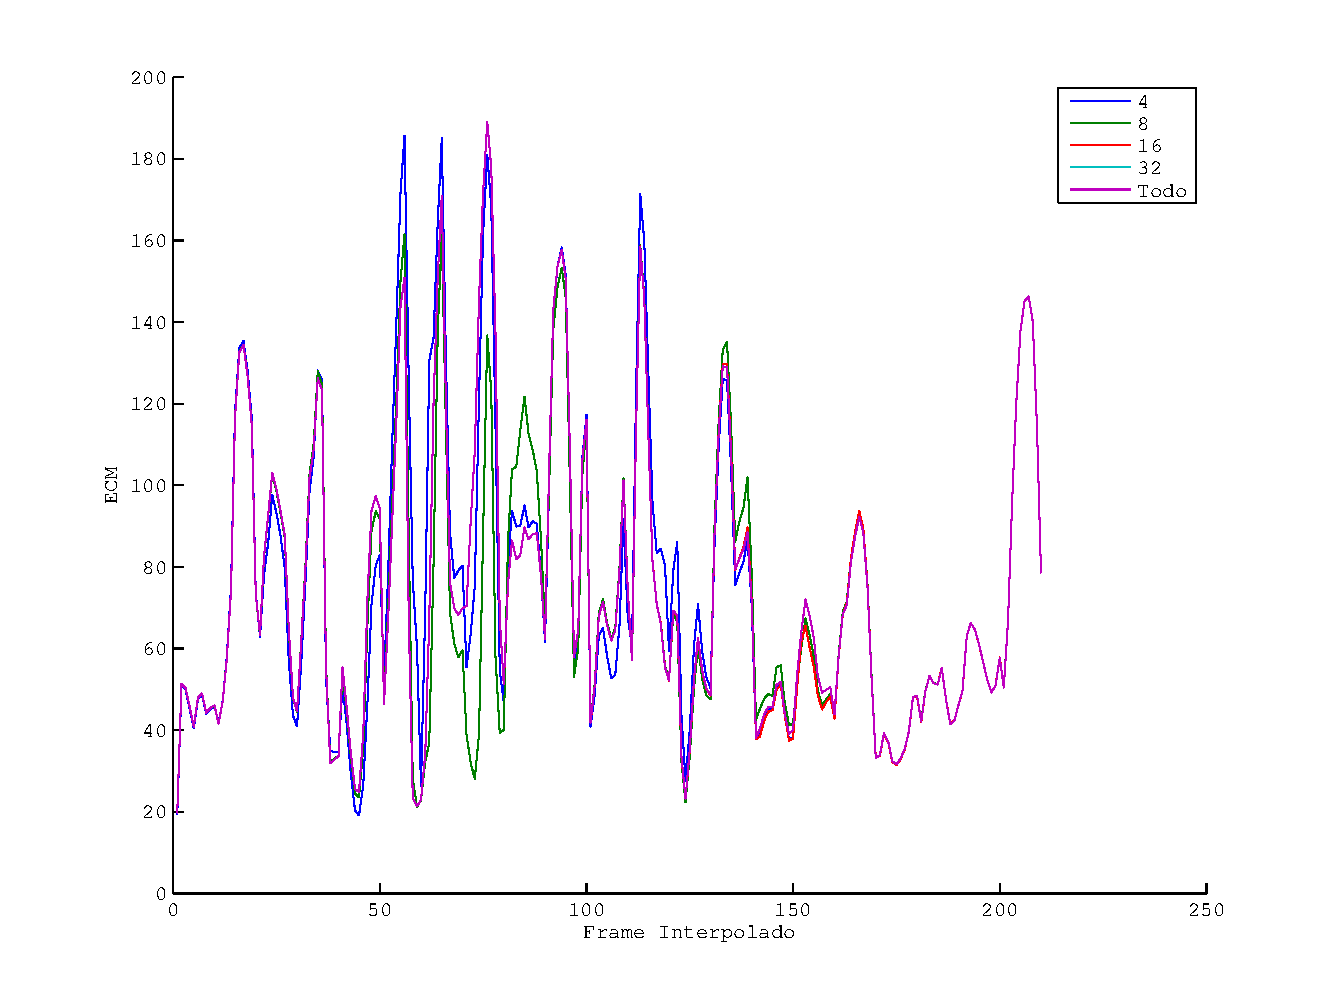
\includegraphics[width=.5\textwidth]{mse_spline-camara_movil-imagen_movil-k10.pdf}
        \label{subfig:movil-movil_spline-mse-k10}
    }
    \subfloat[][PSNR para 10 frames interpolados]{
        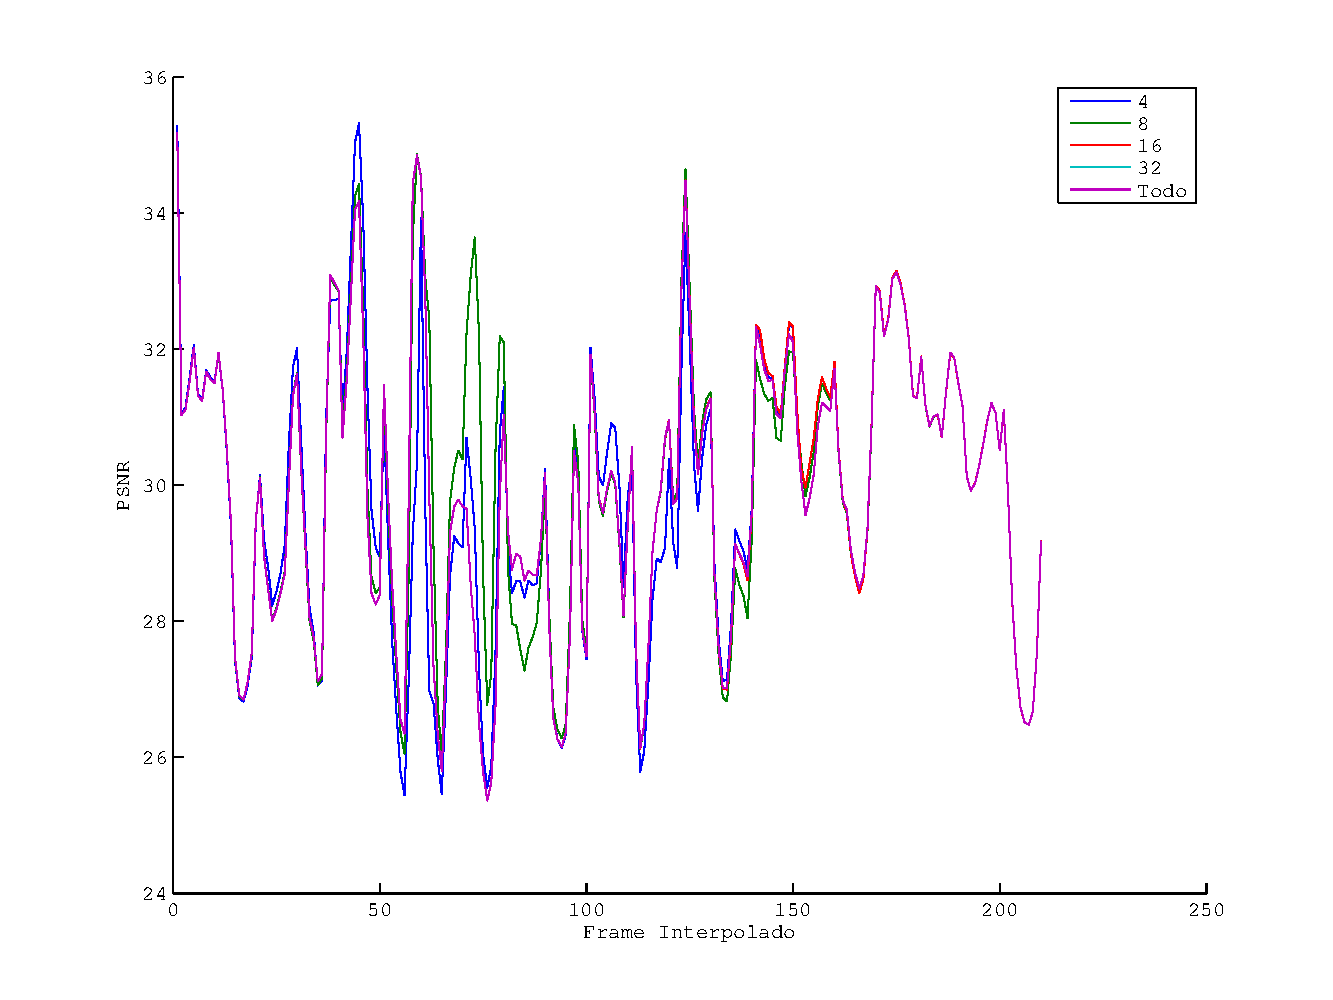
\includegraphics[width=.5\textwidth]{psnr_spline-camara_movil-imagen_movil-k10.pdf}
        \label{subfig:movil-movil_spline-psnr-k10}
    }
    \caption{Comparativa tama\~no de bloque para 10 frames interpolados}
    \label{fig:movil-movil_spline-bloques}
\end{figure}

\par El primer resultado al que llegamos en este experimento es id\'entico al
de los casos de las secciones \ref{subsec:fija-fija} y \ref{subsec:movil-fija}:
el tama\~no de bloque poco parece influir en el error de la estimaci\'on.
Nuevamente observamos en la figura \ref{fig:movil-movil_spline-bloques} como
el ECM y PSNR se solapan frame a frame para todos los tama\~nos de bloque
(salvo algunas secuencias cortas de frames donde alguna de las variantes se
comporta distinto\footnote{Por limitantes de tiempo, no pudimos analizar que
ocurr\'ia en el video de manera de que alg\'un tama\~no de bloque se comportase
de diferente al resto. Intu\'imos que se debe a que el bloque finaliza en medio
de alguna secuencia de frames donde hay mucho movimiento, con lo cual se suma
el error de la transici\'on de un bloque interpolado al siguiente.}).

\par Este comportamiento se ve en todas las variantes de cantidad de frames
interpolados, con lo cual solo se decidi\'o exponer el caso para 10 frames
interpolados.

\begin{figure}[H]
    \centering
    \subfloat[][Valor medio, Desv\'io Est\'andar, M\'aximo y M\'inimo\label{tbl:stats}]{
        \footnotesize
        \setlength{\tabcolsep}{3pt}
        \begin{tabular}{|l|r|r|r|r|}
            \hline
            \textbf{Bloque}& \textbf{Mean}& \textbf{Std}& \textbf{M\'ax}& \textbf{M\'in}\\
            \hline\hline
            4&75.6484& 37.1984& 185.5793& 19.1091\\
            8&72.3007& 34.4053& 161.4246& 19.7056\\
            16&74.3743& 36.0983& 189.0383& 19.7045\\
            32&74.5982& 35.9172& 189.0373& 19.7045\\
            Entero&74.5982& 35.9172& 189.0373& 19.7045\\
            \hline
        \end{tabular}
    }\hspace{10pt}
    \subfloat[][Diferencia M\'axima\label{tbl:difs}]{
        \footnotesize
        \setlength{\tabcolsep}{3pt}
        \begin{tabular}{|l|r|r|r|r|r|}
            \hline
            \textbf{Bloque}& \textbf{vs 4}& \textbf{vs 8}& \textbf{vs 16}& \textbf{vs 32}& \textbf{vs Entero}\\
            \hline\hline
            \textbf{4}&0& 93.5795& 63.3860& 63.3862& 63.3862\\
            \textbf{8}&26.6351& 0& 31.9637& 31.9555& 31.9555\\
            \textbf{16}&32.9524& 106.3786& 0& 1.4232& 1.4232\\
            \textbf{32}&32.9537& 106.3761& 7.7375& 0& 0\\
            \textbf{Entero}&32.9537& 106.3761& 7.7375& 0& 0\\
            \hline
        \end{tabular}
    }
    \caption{Comparativa ECM seg\'un tama\~no de bloque}
\end{figure}

\par Continuando, observamos en el cuadro \ref{tbl:stats} como los valores
estad\'isticos de la m\'etrica del ECM valida la aseveraci\'on de que el
tama\~no de bloque no pareciera influir. Todos los valores obtenidos son muy
similares (y en el caso de bloque de 32 frames y video entero, iguales).

\par A diferencia de los casos previos, observamos al considerar las diferencias
m\'aximas para un mismo frame (cuadro \ref{tbl:difs}) que, salvo en el caso
de tama\~no de bloque 4, un menor tama\~no de bloque tiene una diferencia menor
respecto (es decir, el frame en el cual sus alternativas estiman mucho mejor)
que a la inversa. El caso del tama\~no 4 es la excepci\'on, siendo este el peor
caso al considerar esta diferencia. Esto de alguna manera nos parece una
caracter\'istica que puede inclinar la balanca por un tama\~no de bloque 8, ya
que del an\'alisis de la figura \ref{fig:movil-movil_spline-mse_estadisticas} se
reconfirma que el tama\~no de bloque poco afecta a los valores medios del ECM a
lo largo de todos los frames del video.

\par Continuando con los resultados expuestos en la figura
\ref{fig:movil-movil_spline-mse-estadisticas}, observamos nuevamente que el
ECM medio se incrementa a medida que se interpolan m\'as cuadros, como se hab\'ia
propuesto en las hip\'otesis iniciales. Sin embargo, al observar el m\'inimo
error cometido es interesante destacar que el comportamiento es m\'as err\'atico.
Se observa que la mejor aproximaci\'on de un \'unico frame se obtiene al
interpolar de a 5 frames, seguido del caso de 10 frames. Queda para futuros
experimentos determinar el porque de este comportamiento.

\begin{figure}[H]
    \centering
    \subfloat[][Valor Medio]{
        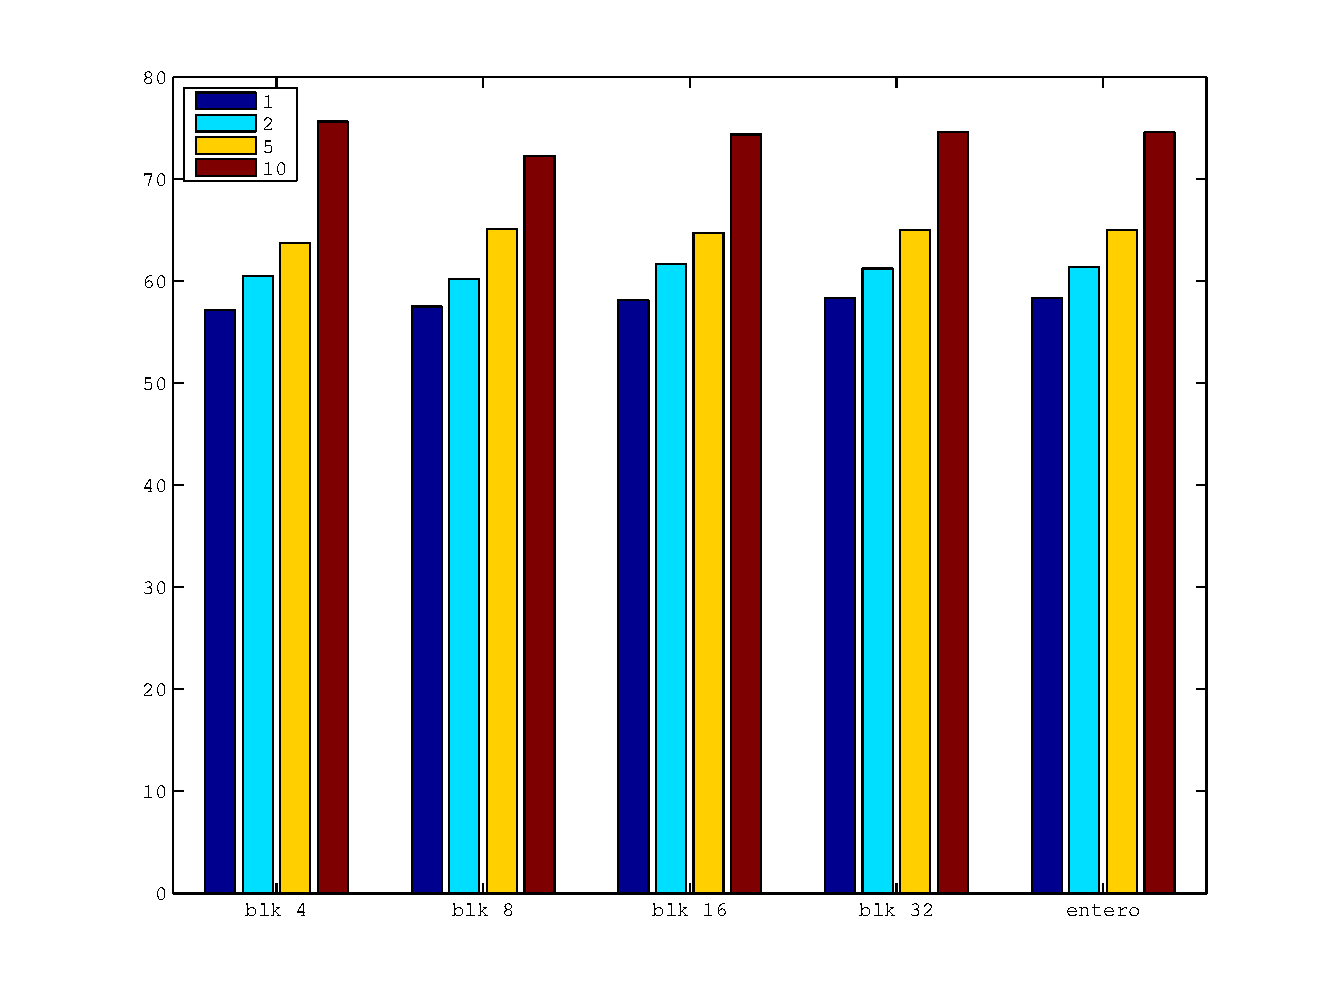
\includegraphics[width=.5\textwidth]{camara_movil-imagen_movil-mean_spline.pdf}
    }
    \subfloat[][Desv\'io Est\'andar]{
        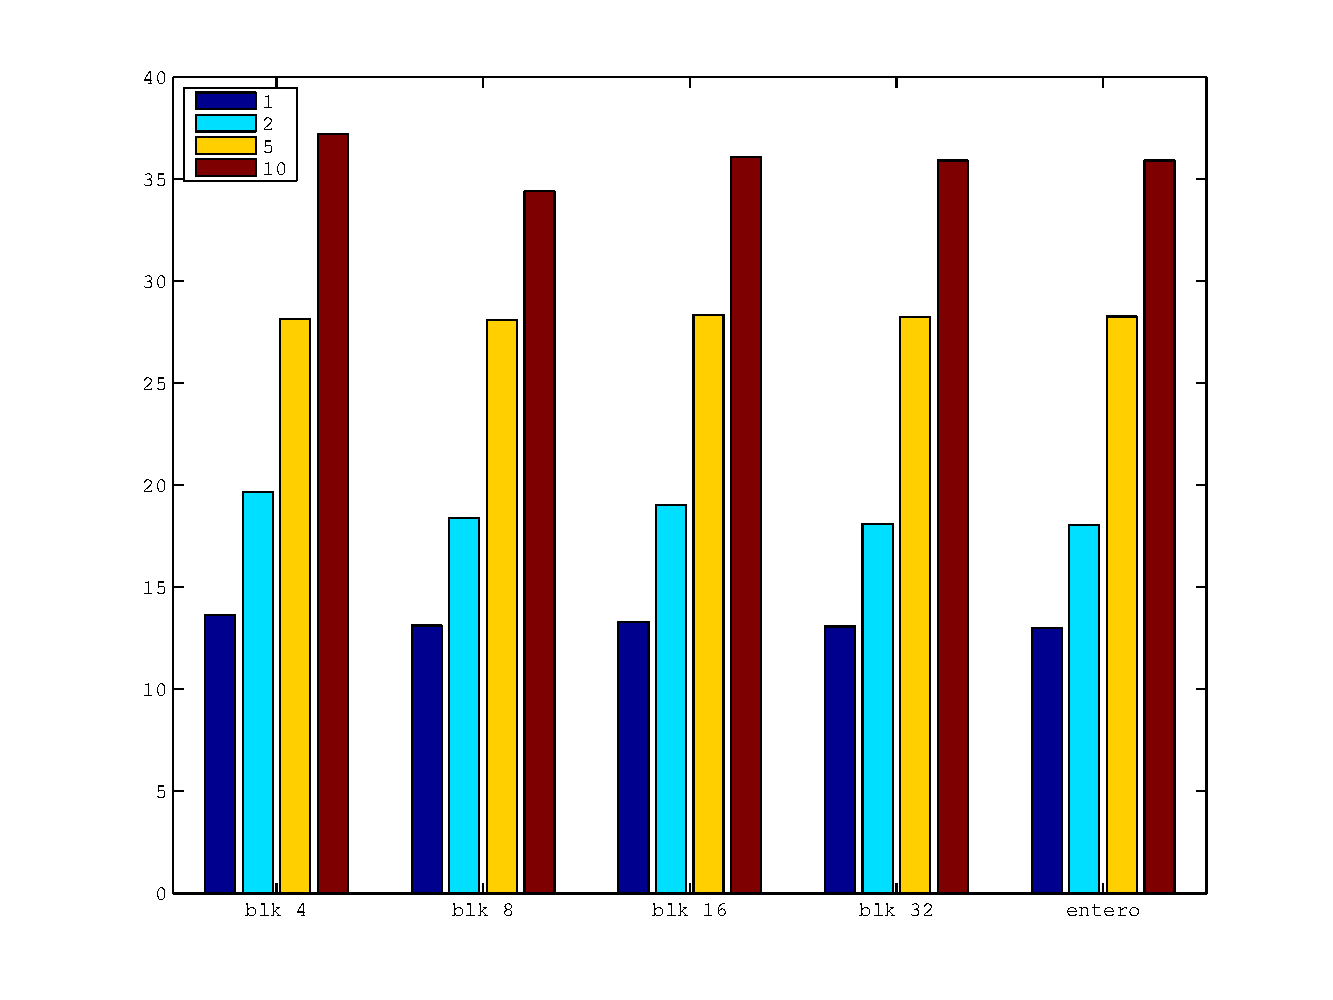
\includegraphics[width=.5\textwidth]{camara_movil-imagen_movil-std_spline.pdf}
    }\\
    \subfloat[][M\'aximo]{
        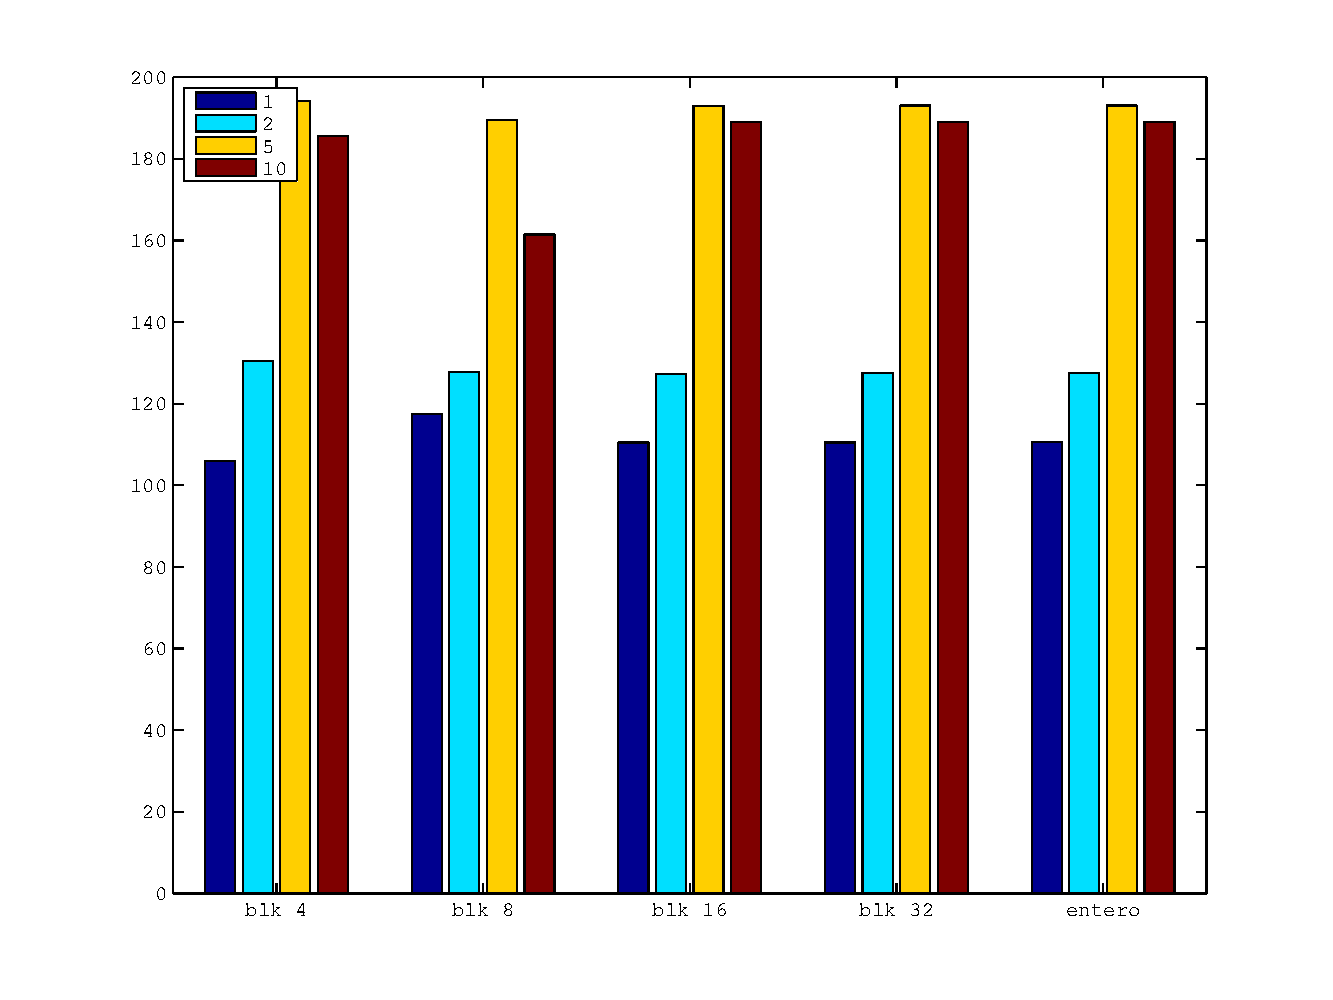
\includegraphics[width=.5\textwidth]{camara_movil-imagen_movil-max_spline.pdf}
    }
    \subfloat[][M\'inimo]{
        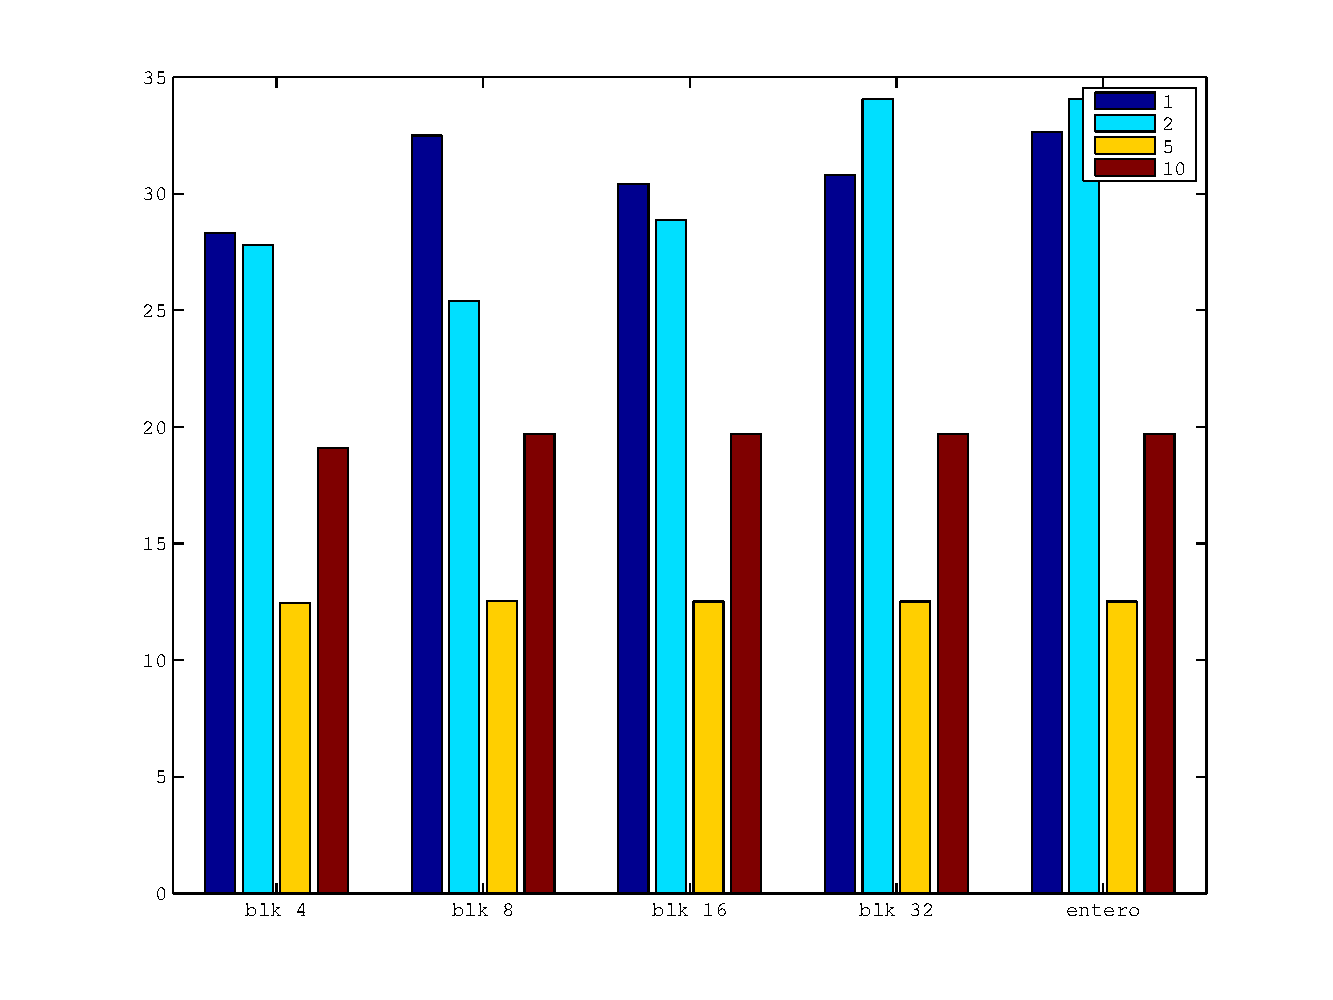
\includegraphics[width=.5\textwidth]{camara_movil-imagen_movil-min_spline.pdf}
    }
    \caption{Est\'adisticas ECM Seg\'un Frames Interpolados - Spline}
    \label{fig:movil-movil_spline-mse_estadisticas}
\end{figure}

\par Por \'ultimo, pasamos al video comparador de diferencias entre frames
para el caso de 10 frames interpolados (el caso de mayor desv\'io est\'andar) y
tama\~no de bloque 8 (por los motivos ya
explicados)\footnote{\url{https://drive.google.com/open?id=0B0RfkWV-4-XqUHA0Y0F3WmY2a0k}},
con el objetivo de identificar las regiones que m\'as aportan al ECM de la
interpolaci\'on. En la figura \ref{fig:movil-movil_spline-heatmap} se puede
observar una captura representativa de dicho video.

\begin{figure}[H]
    \centering
    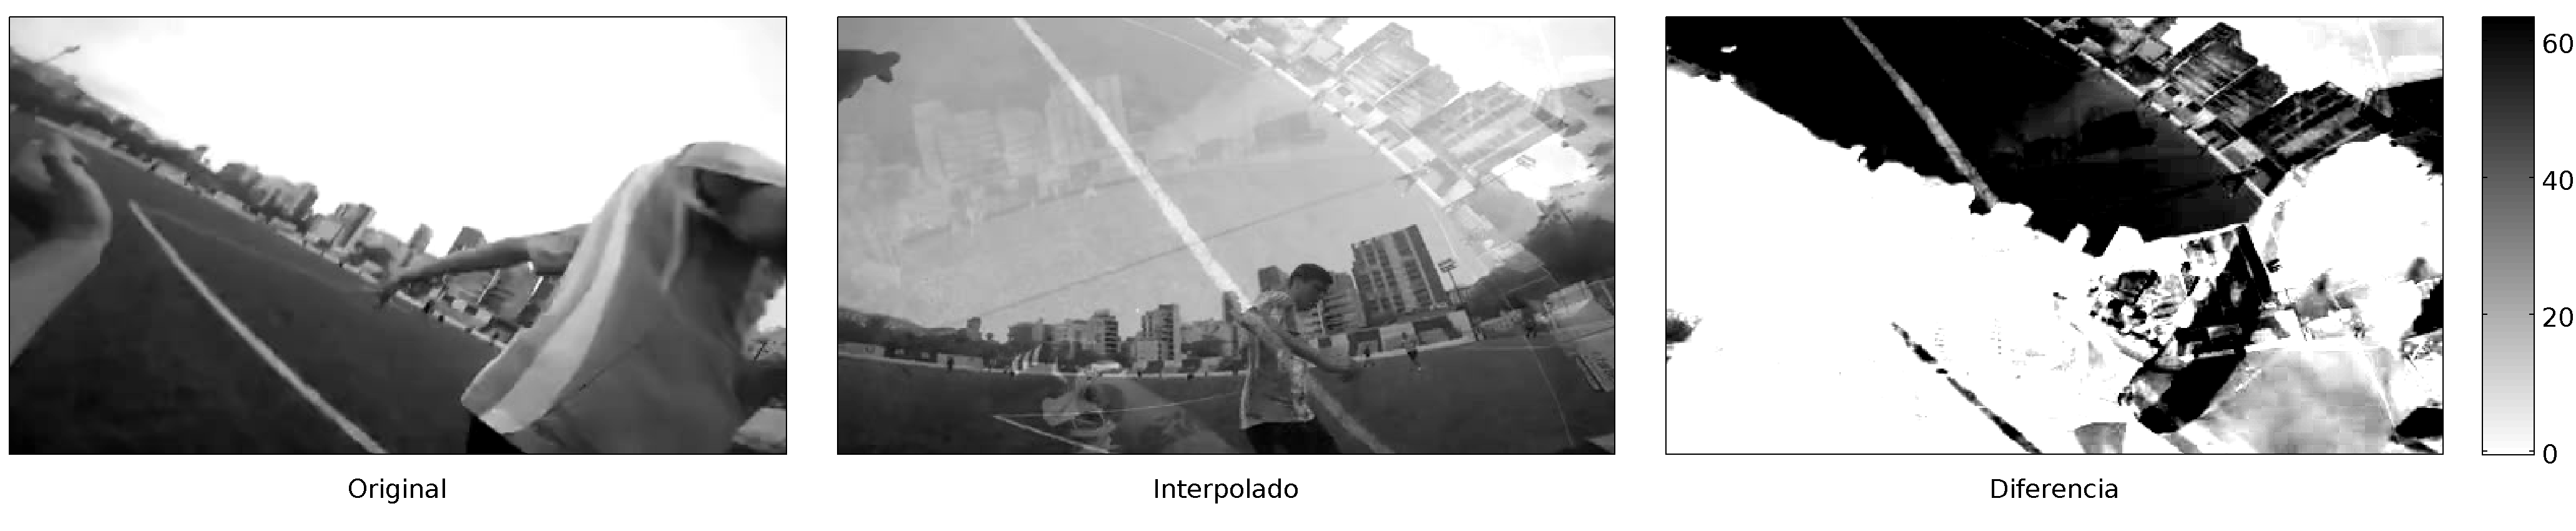
\includegraphics[width=\textwidth]{camara_movil-imagen_movil-spline-k10-blk8.png}
    \label{fig:movil-movil_spline-heatmap}
    \caption{Regi\'on peor aproximada por la interpolaci\'on por spline}
\end{figure}

\par Lo que se observa a lo largo de este video es, b\'asicamente, que todo
aporta al error. La filmaci\'on est\'a en movimiento constante y err\'atico, y
en algunos casos los movimientos de la c\'amara son muy bruscos/repentinos,
cambiando el \'angulo de filmaci\'on de forma amplia en pocos frames. Todo esto
lleva a que el error est\'e distribu\'ido (y en valores altos) a lo largo de
todo el frame, m\'as all\'a de que dependiendo la parte del video sea una
regi\'on u otra la que m\'as aportan. C\'omo t\'ermino general, observamos que
cuando una regi\'on presenta mucho m\'as error que el resto, se debe a que
fruto del movimiento de la c\'amara y lo que se est\'a filmando, hubo un cambio
abrupto de forma y tonalidad en la regi\'on que presenta el error. En el
ejemplo de la figura expuesta, el \'angulo de la c\'amara cambi\'o
repentinamente rotando mayormente en un plano $XY$\footnote{Utilizando la
convenci\'on de que la profundidad es el eje $Z$, el ancho de la im\'agen el
eje $X$ y el alto el $Y$}, haciendo que la interpolaci\'on comienze a
''superponer'' dos im\'agenes que no coinciden en mucho (como se ve en el frame
''interpolado'' de la figura).  Luego, se observa que la regi\'on
correspondiente al verde del terreno de juego es la que menos error presenta,
posiblemente ya que en frame al que se est\'a transicionando esa misma regi\'on
tambi\'en represente parte del terreno de juego, que suele tener un color
tendiendo a uniforme. Mientras tanto, todas las dem\'as regiones de la im\'agen
presentan un error alt\'isimo.

%---------------------------------------------------------------
\subsubsection{Interpolaci\'on Lineal}

\begin{figure}[H]
    \centering
    \subfloat[][Valor Medio]{
        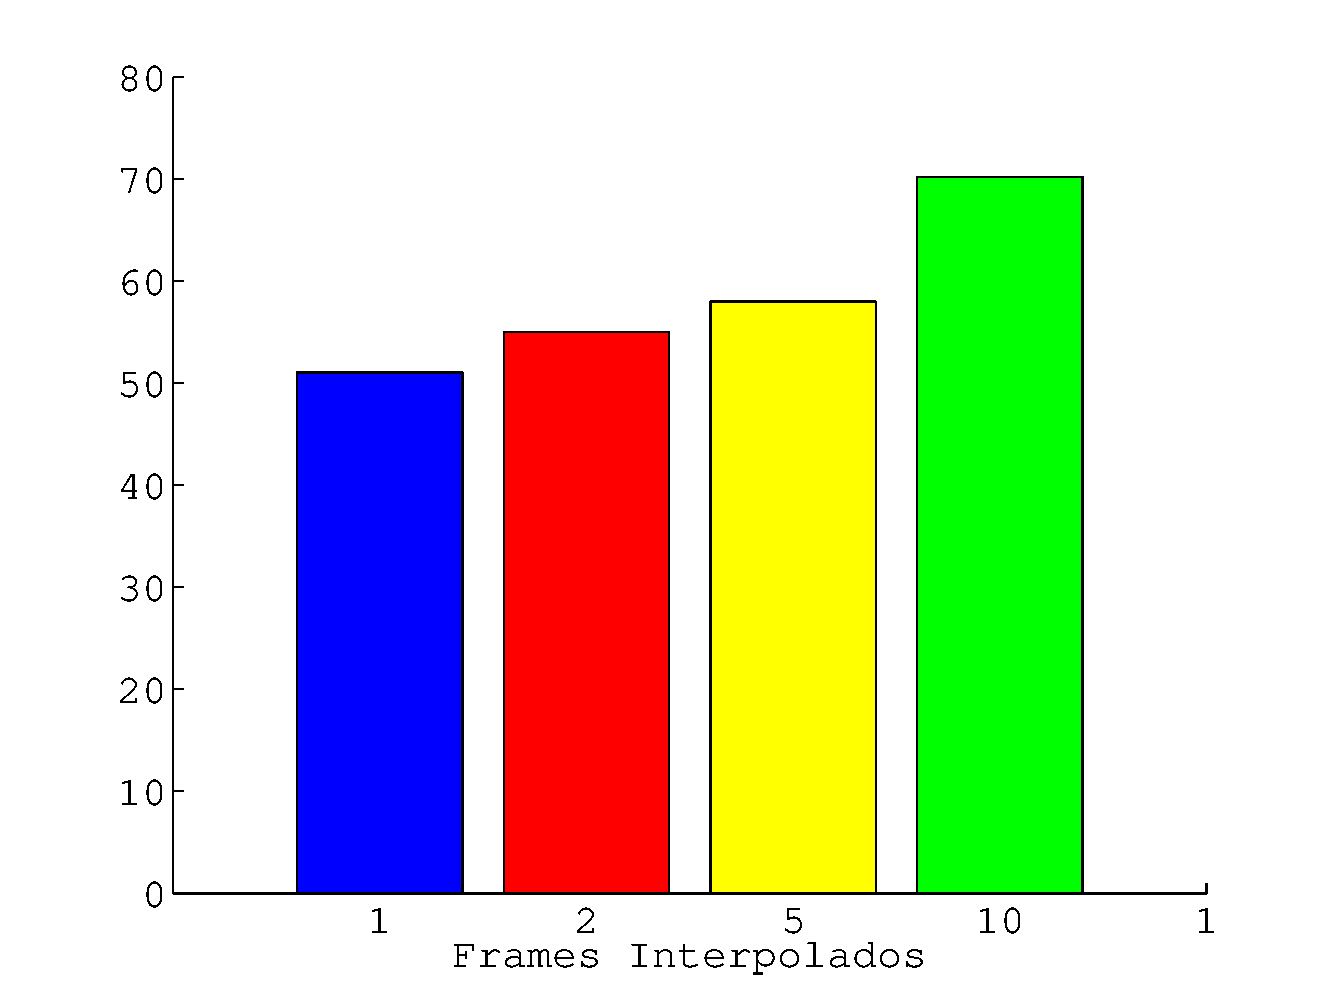
\includegraphics[width=.25\textwidth]{camara_movil-imagen_movil-mean_lineal.pdf}
    }
    \subfloat[][Desv\'io Est\'andar]{
        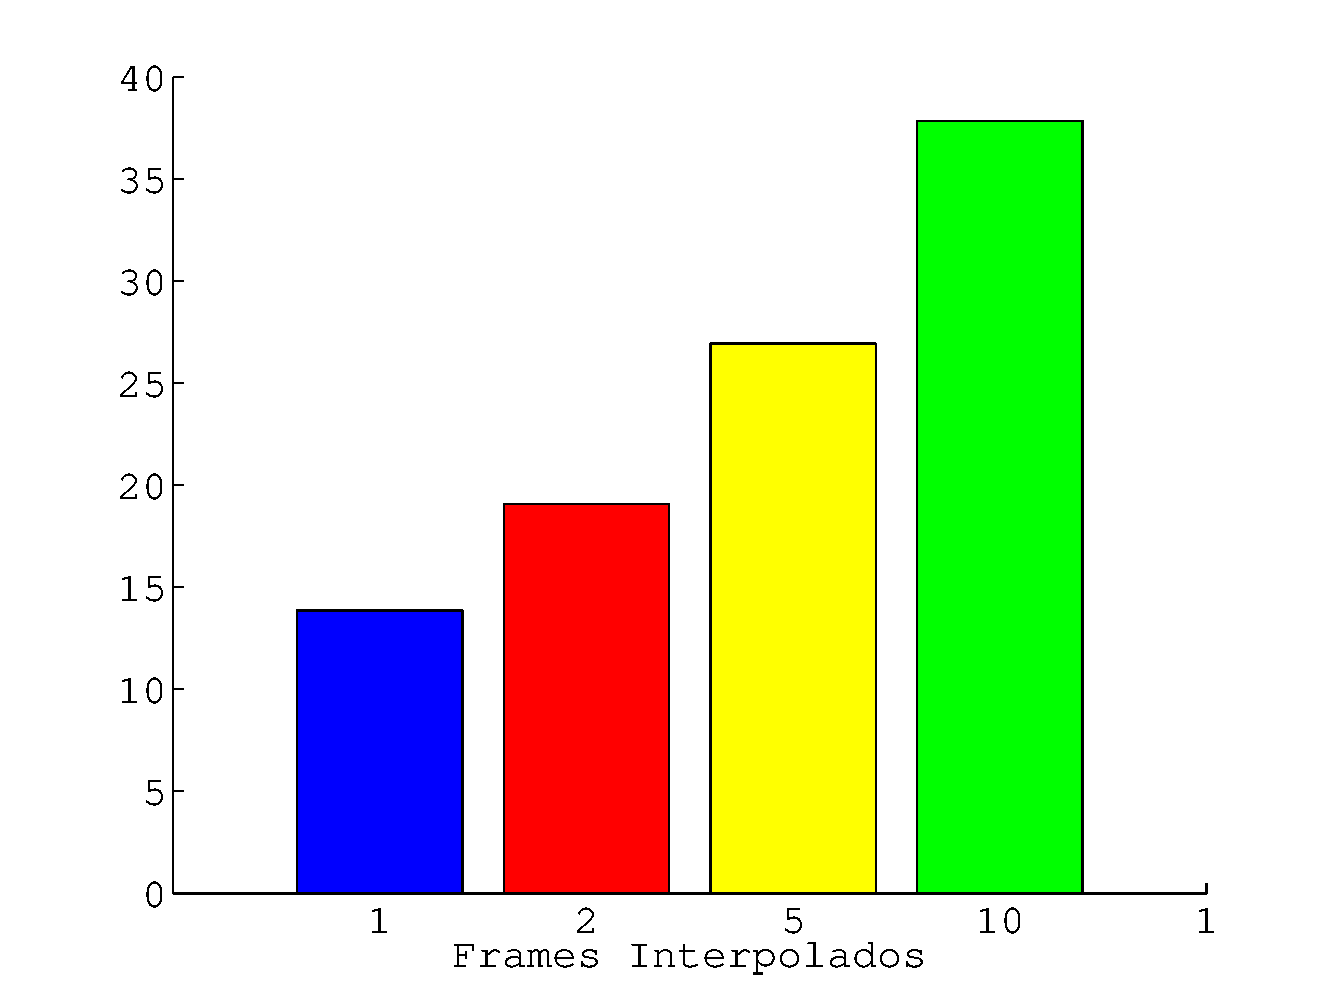
\includegraphics[width=.25\textwidth]{camara_movil-imagen_movil-std_lineal.pdf}
    }
    \subfloat[][M\'aximo]{
        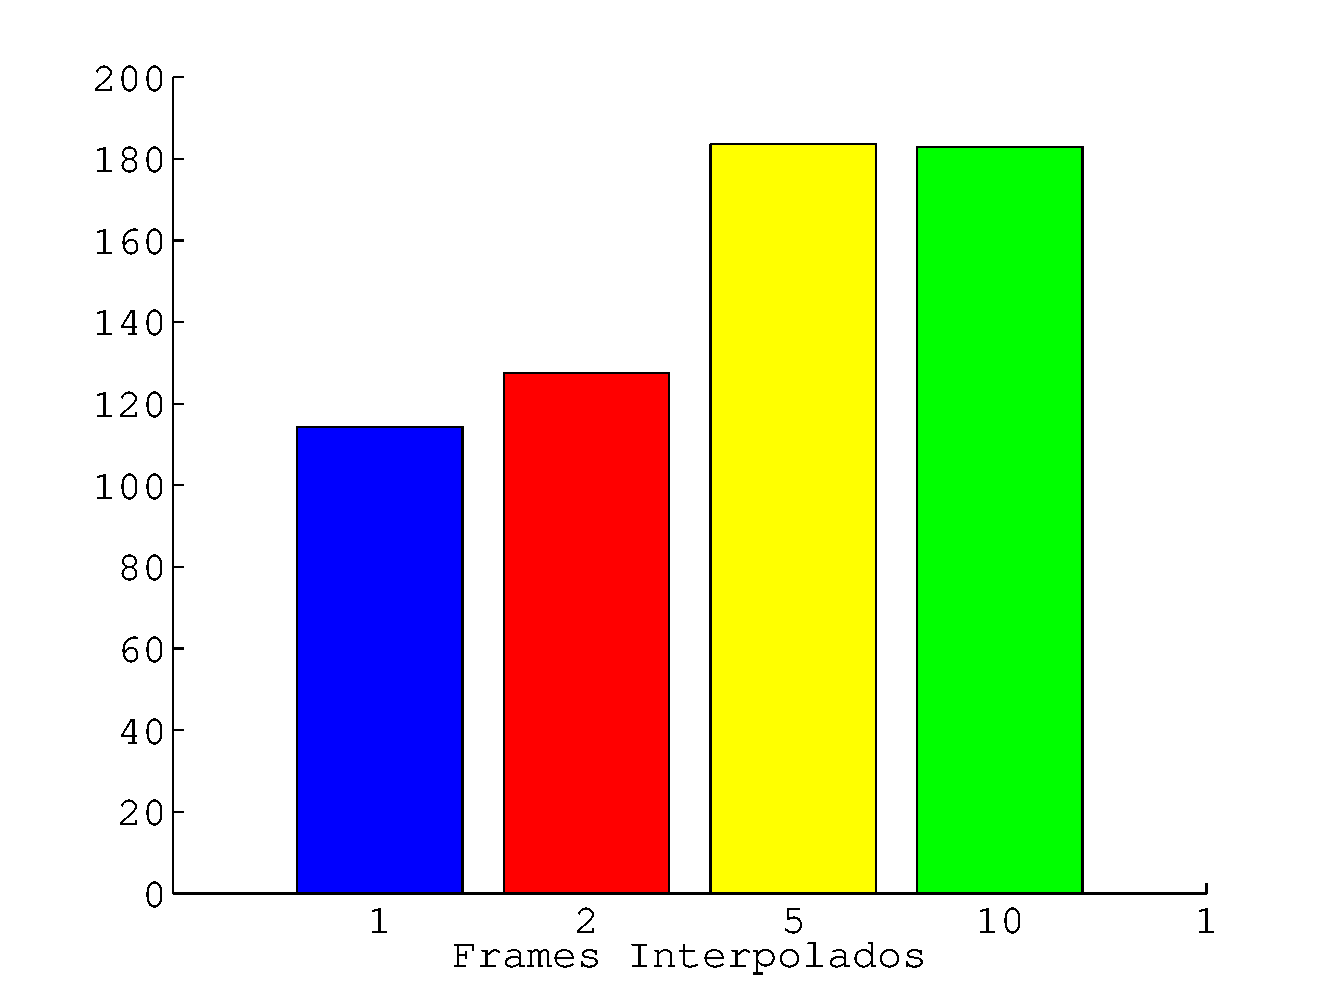
\includegraphics[width=.25\textwidth]{camara_movil-imagen_movil-max_lineal.pdf}
    }
    \subfloat[][M\'inimo]{
        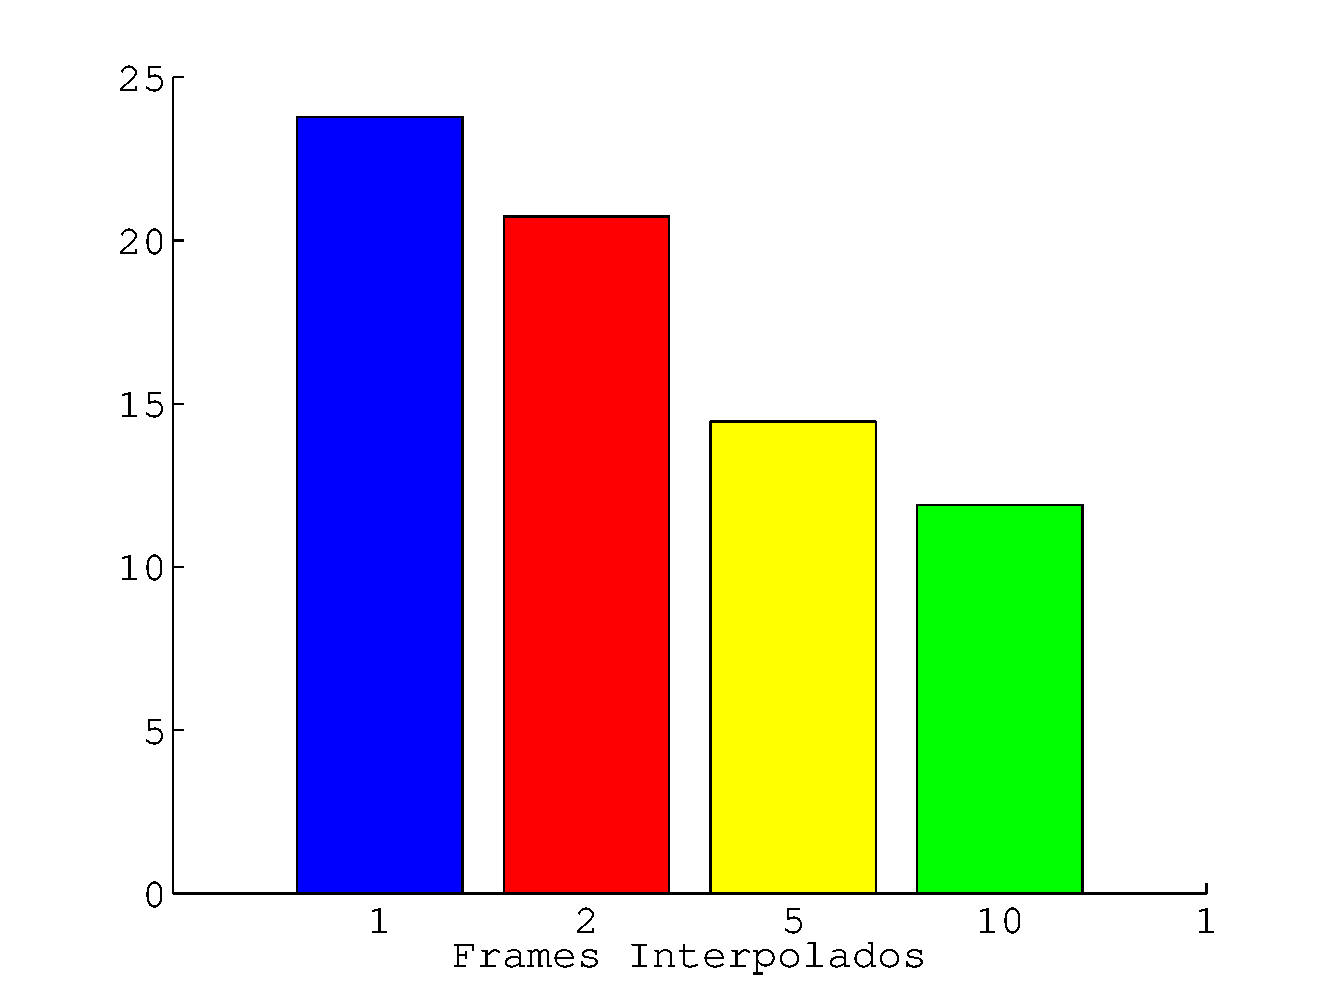
\includegraphics[width=.25\textwidth]{camara_movil-imagen_movil-min_lineal.pdf}
    }
    \caption{Est\'adisticas ECM Seg\'un Frames Interpolados - M\'etodo Lineal}
    \label{fig:movil-movil_lineal-mse_estadisticas}
\end{figure}

\par La observaci\'on de los resultados est\'adisticos (figura
\ref{fig:movil-movil_lineal-mse_estadisticas})confirma nuevamente la gran
mayor\'ia de las hip\'otesis planteadas. Por un lado se tiene que el valor
medio del ECM se incrementa a medida que lo hace la cantidad de frames
interpolados, como as\'i tambi\'en lo hace el frame peor estimado (m\'aximo
ECM). Sin embargo, observamos un comportamiento inesperado en cuanto a la mejor
aproximaci\'on (ECM m\'inimo). Se ve como la mejor aproximaci\'on se da a medida
que se interpolan m\'as y m\'as frames. De alguna manera, la cantidad de
movimiento del video hace que al tener frames originales cercanos pero muy
distintos, el m\'etodo no estime mejor que cuando estos est\'an m\'as
distanciados (es decir, m\'as frames entre estos deben ser generados
artificialmente). Esto se puede deber a que al interpolar entre frames muy
distintos cercanos en el orden de reproducci\'on original, se obtenga un
polinomio interpolador lineal de orden 1 muy abrupto, y podr\'ia ocurr\'i que
en realidad el frame interpolado en el video original en realidad est\'e mucho
m\'as cerca de algun de los frames que se usan para calcular el polinomio
interpolador.

%\par Continuando, observamos que el desv\'io est\'andar tambi\'en aumenta
%conforme lo hace la cantidad de frames interpolados. Para entender un poco m\'as

%\begin{figure}[H]
%    \centering
%    \subfloat[][PSNR para 1 frame interpolado]{
%        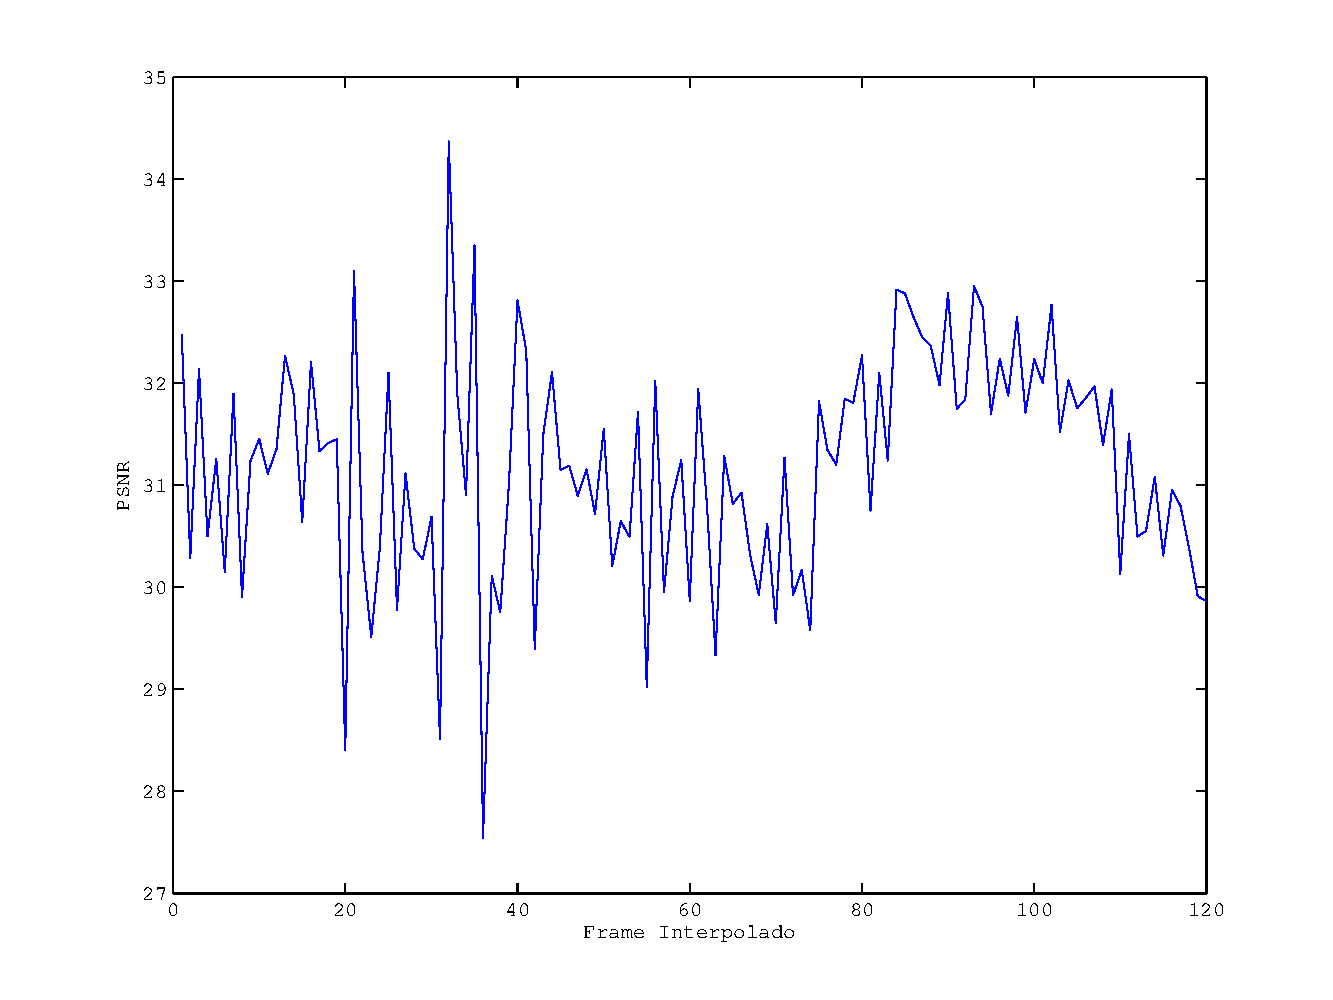
\includegraphics[width=.5\textwidth]{camara_movil-imagen_movil-LINEAL-psnr-k1.pdf}
%        \label{subfig:movil-movil_lineal-psnr-k1}
%    }
%    \subfloat[][PSNR para 10 frames interpolados]{
%        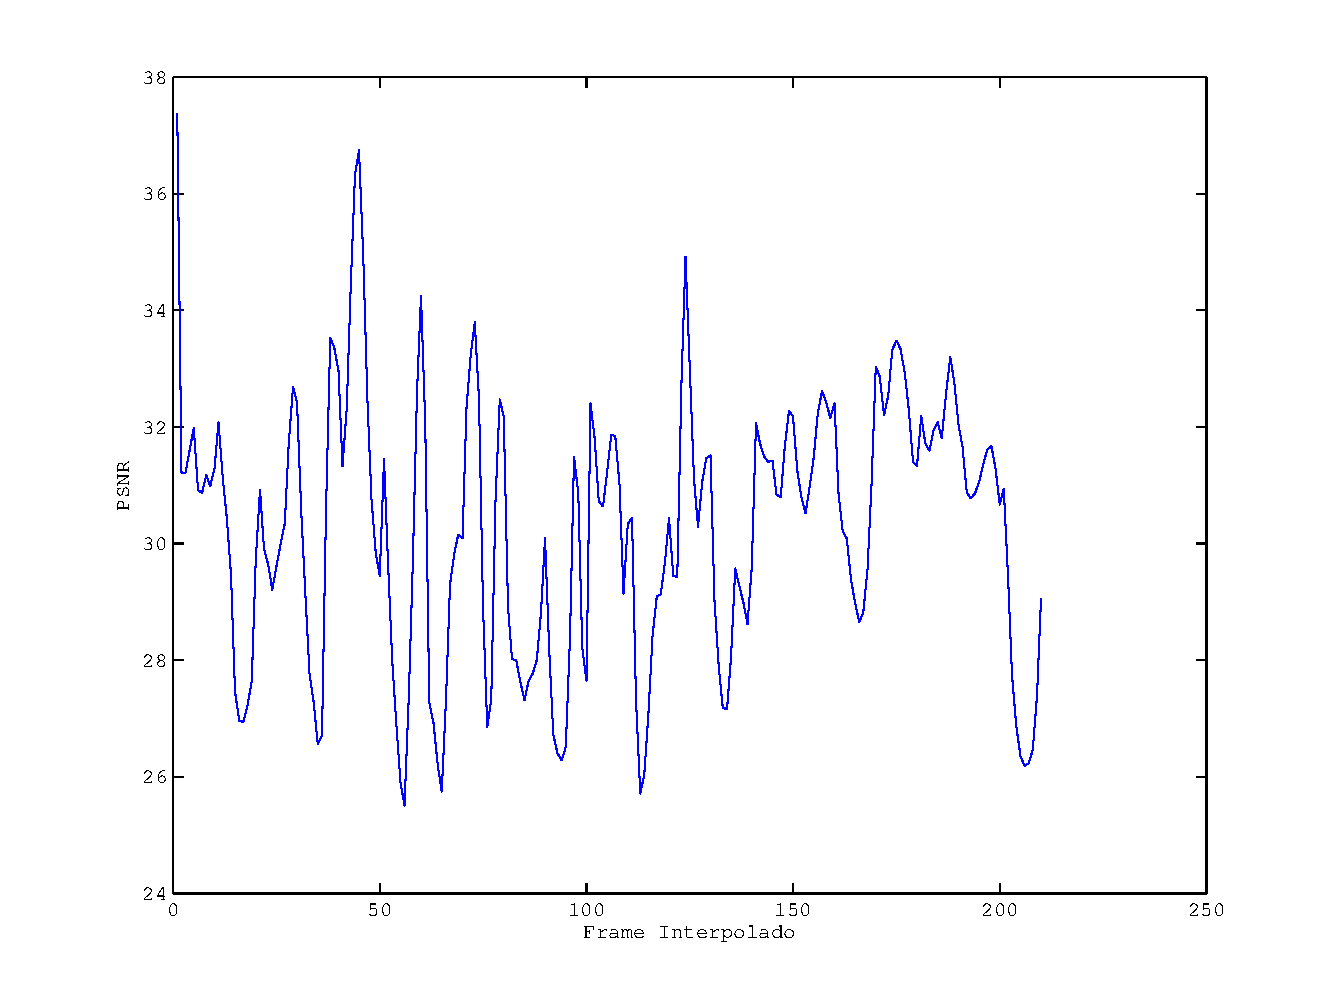
\includegraphics[width=.5\textwidth]{camara_movil-imagen_movil-LINEAL-psnr-k10.pdf}
%        \label{subfig:movil-movil_lineal-psnr-k10}
%    }
%    \caption{Comparativa seg\'un cantidad de bloques interpolados}
%    \label{fig:movil-movil_lineal-psnr}
%\end{figure}

\par Por \'ultimo, antes de pasar al m\'etodo restante, en cuanto al video
comparador para 10 frames
inteprolados\footnote{\url{https://drive.google.com/open?id=0B0RfkWV-4-XqLUZ2aWdMT3hNSDg}}
se obtienen las mismas conclusiones que para el caso de spline.

%---------------------------------------------------------------
\subsubsection{Vecino m\'as Cercano}

\begin{figure}[H]
    \centering
    \subfloat[][Valor Medio]{
        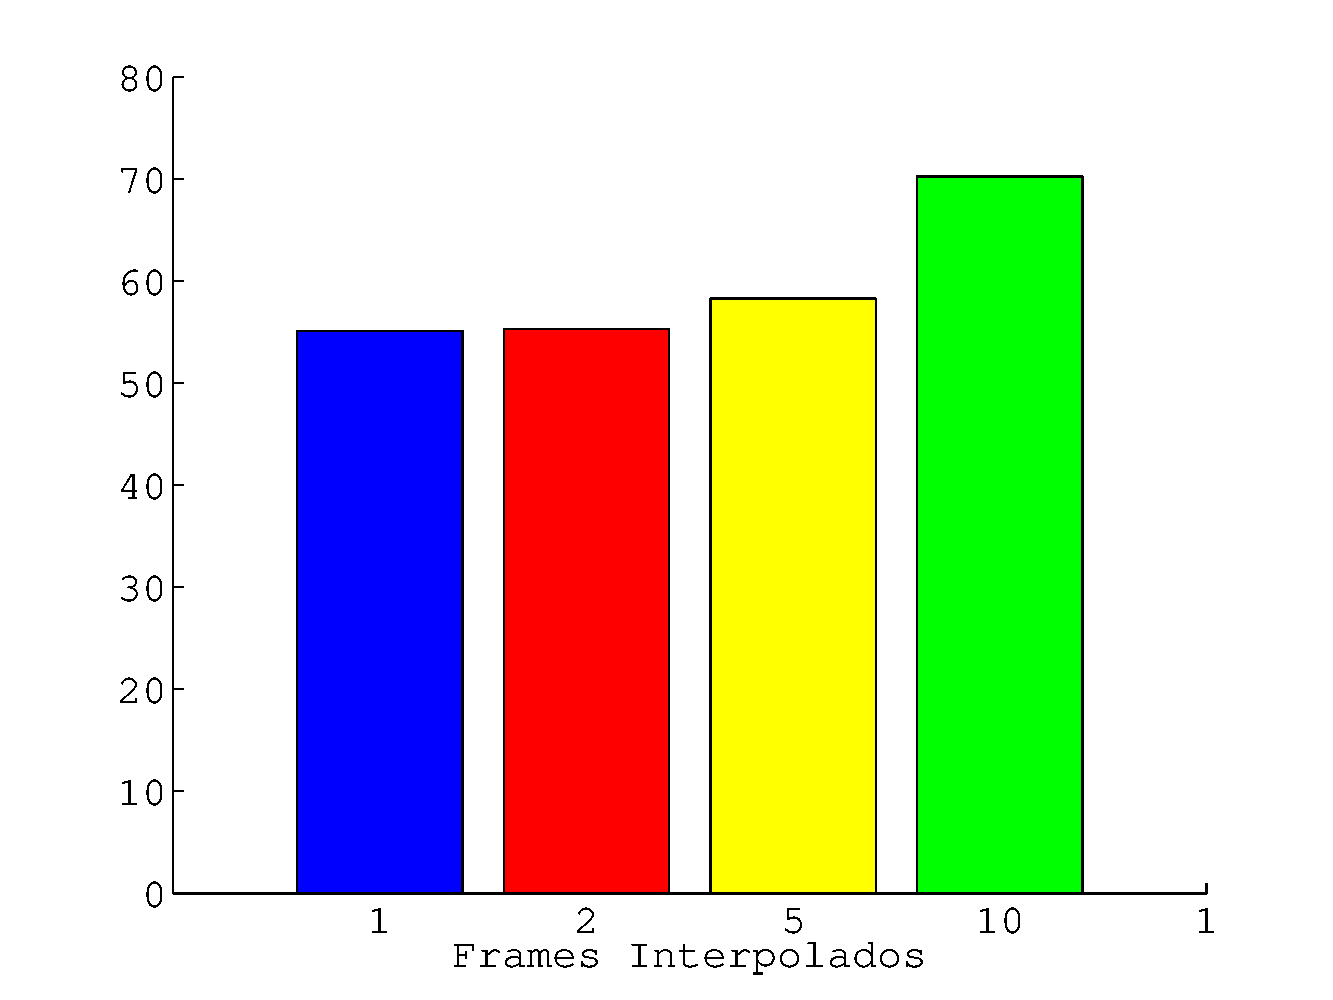
\includegraphics[width=.25\textwidth]{camara_movil-imagen_movil-mean_vecino.pdf}
    }
    \subfloat[][Desv\'io Est\'andar]{
        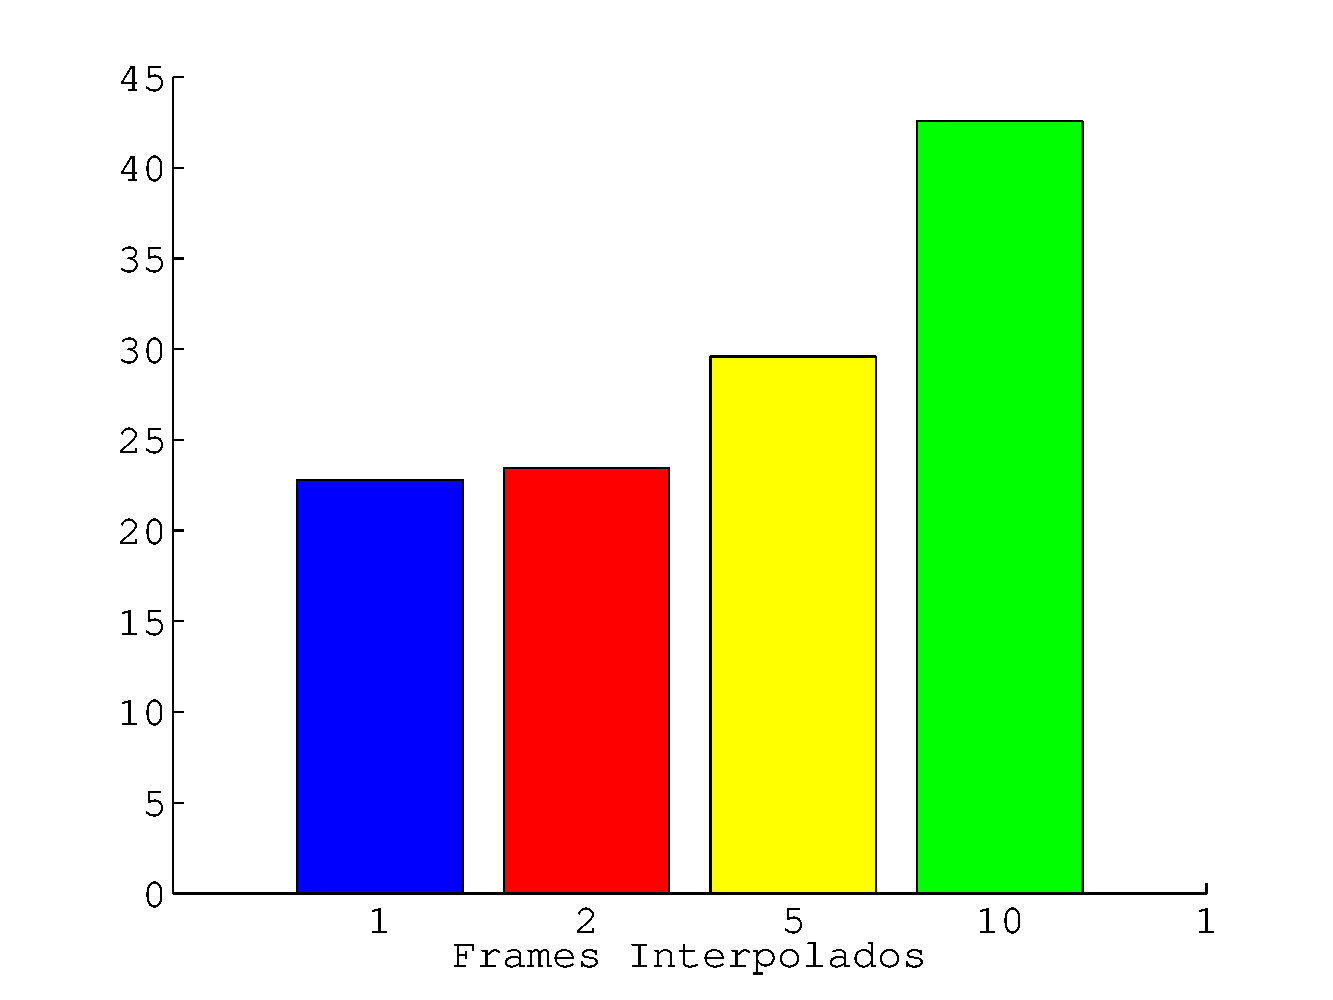
\includegraphics[width=.25\textwidth]{camara_movil-imagen_movil-std_vecino.pdf}
    }
    \subfloat[][M\'aximo]{
        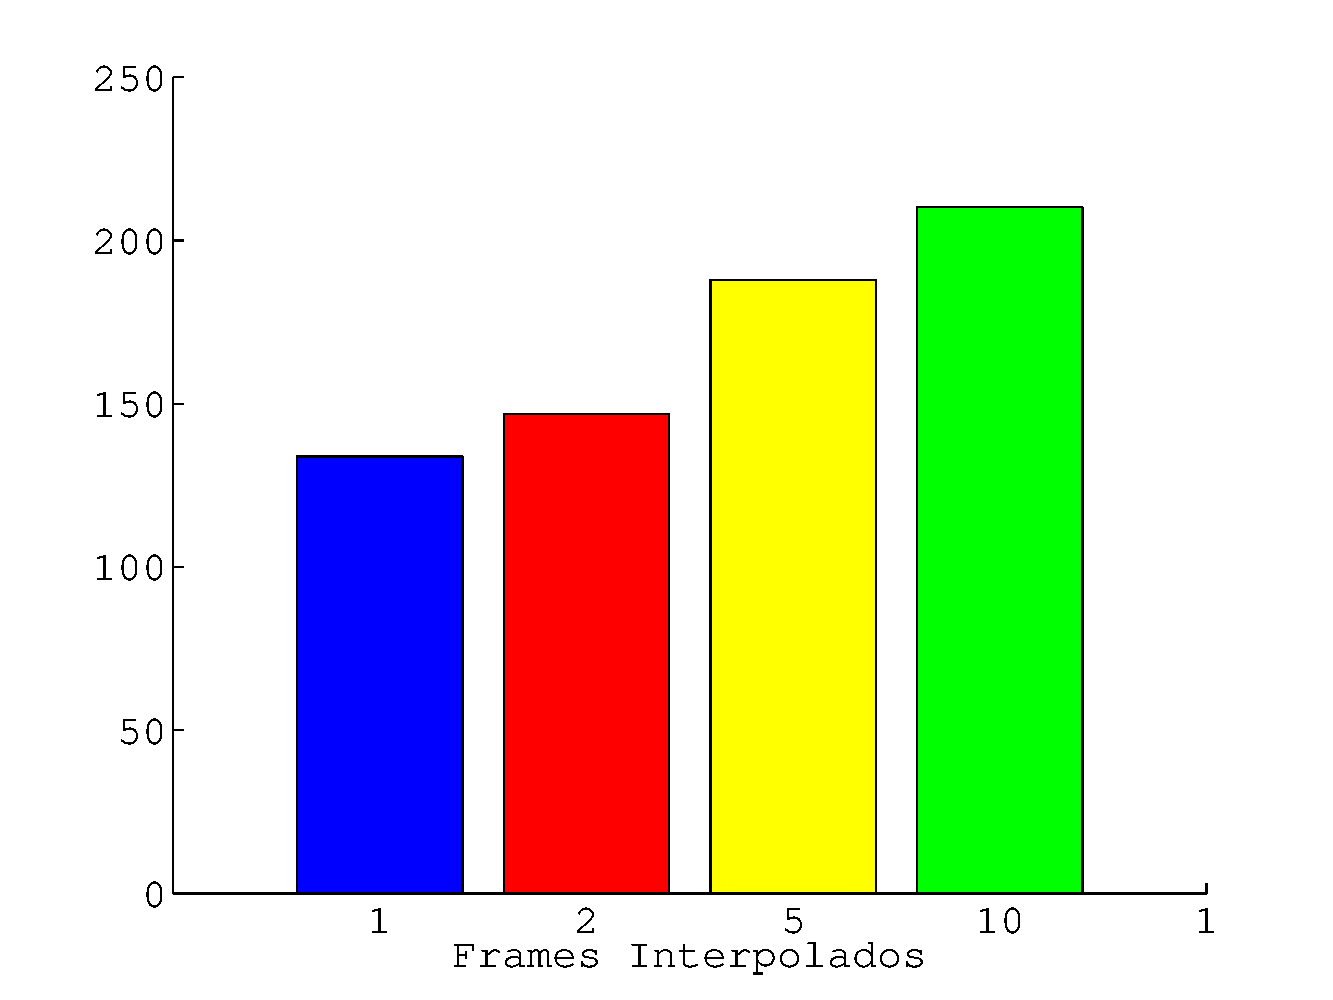
\includegraphics[width=.25\textwidth]{camara_movil-imagen_movil-max_vecino.pdf}
    }
    \subfloat[][M\'inimo]{
        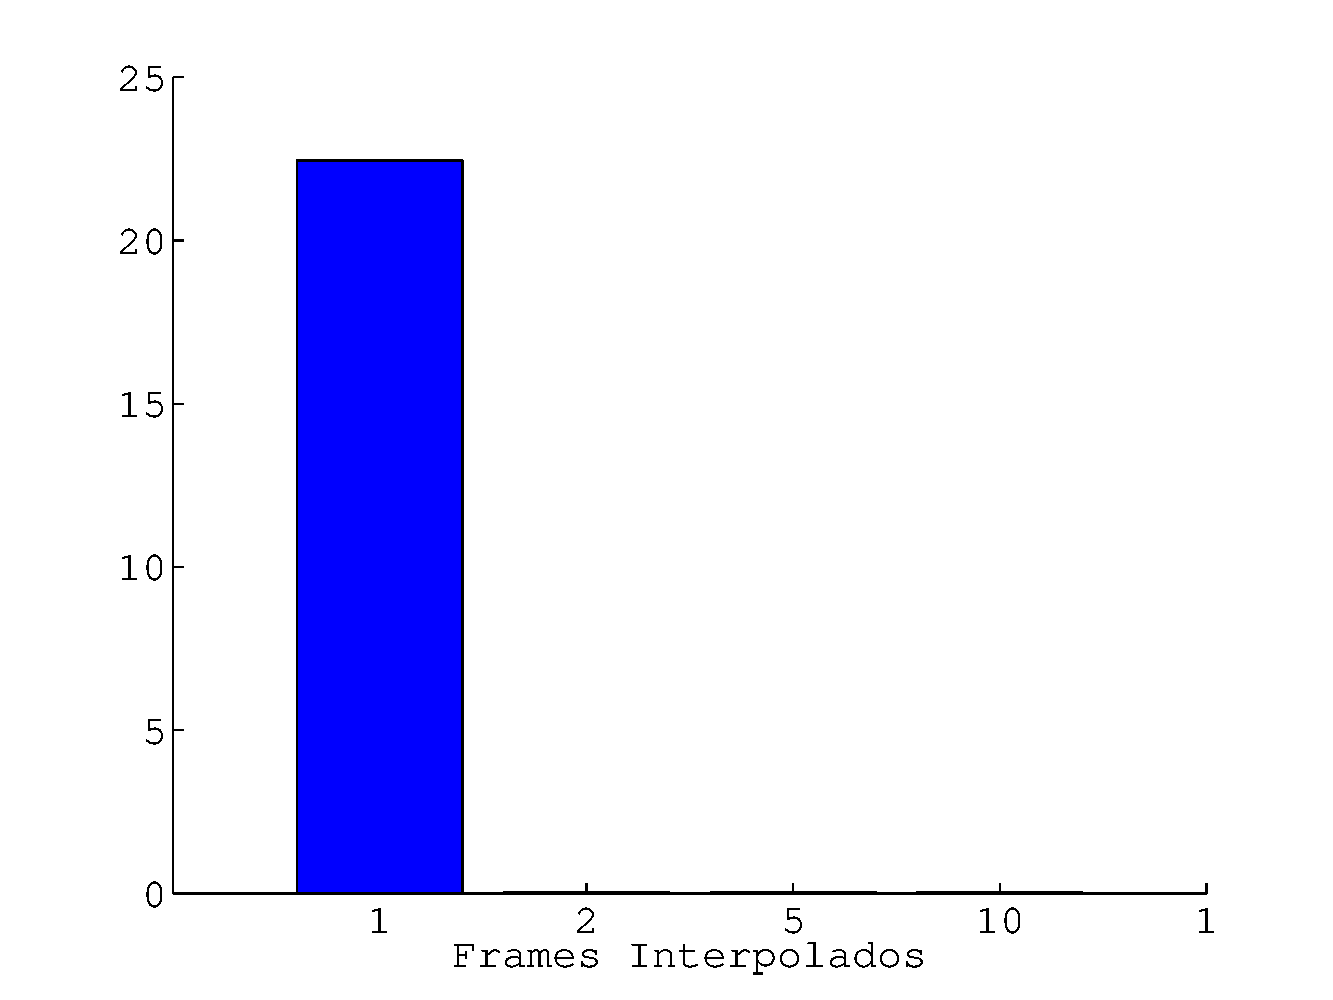
\includegraphics[width=.25\textwidth]{camara_movil-imagen_movil-min_vecino.pdf}
    }
    \caption{Est\'adisticas ECM Seg\'un Frames Interpolados - M\'etodo Vecino m\'as Cercano}
    \label{fig:movil-movil_vecino-mse_estadisticas}
\end{figure}

\par Los resultados obtenidos a partir de la experimentaci\'on de este m\'etodo
no difieren del caso previo para interpolaci\'on l\'ineal, cumpli\'endose las
hip\'otesis planteadas\footnote{¿O ya les podemos decir profec\'ias?}. E
incluso se puede observar que ocurre lo mismo respecto del m\'inimo error
cometido que en el experimento previo (secci\'on
\ref{subsubsec:movil-fija_vecino}), aunque en este caso ocurre a la inversa. Es
decir, en el caso.

\par Recordando esto \'ultimo, lo que se observ\'o es que debido a la decisi\'on
tomada de que frame considerar el \emph{vecino m\'as cercano} en caso de que el
mismo est\'e a igual distancia de reproducci\'on que los frames originales que
se usan calcular la interpolaci\'on. A diferencia del experimento previo, donde
al interpolar un \'unico frame por cada par de frames del video se obten\'ia un
error m\'inimo menor pues la estimaci\'on conseguida para el primer frame generado
artificialmente fruto de utilizar el frame posterior en
la reproducci\'on era mejor que utilizar el frame previo en la reproducci\'on (que
es el que terminaban usando las variantes de 2, 5 y 10 frames interpolados), aqu\'i
ocurre lo contrario. Utilizar el frame previo en la reproducci\'on (caso de 2, 5
y 10 frames interpolados) nos dan ECM m\'inimo mucho menor a no utilizarlo. Se
observa en la figura \ref{fig:movil-movil_vecino-psnr} que justamente es el
primer frame interpolado de esta manera el que es el m\'inimo para estas
variantes.

\begin{figure}[H]
    \centering
    \subfloat[][PSNR para 1 frame interpolado]{
        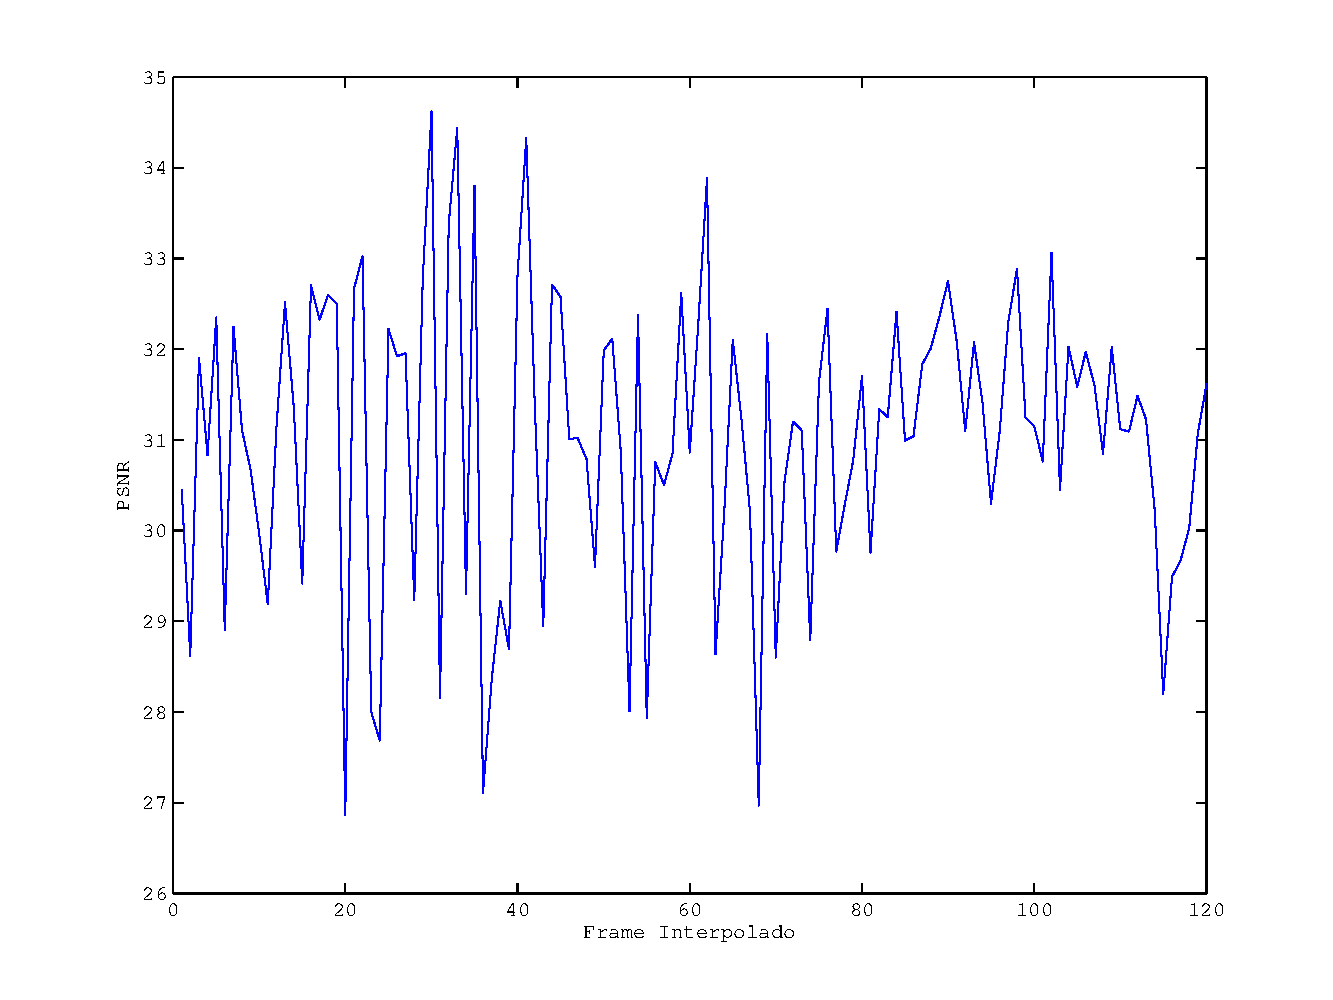
\includegraphics[width=.5\textwidth]{camara_movil-imagen_movil-VECINO-psnr-k1.pdf}
        \label{subfig:movil-movil_vecino-psnr-k1}
    }
    \subfloat[][PSNR para 10 frames interpolados]{
        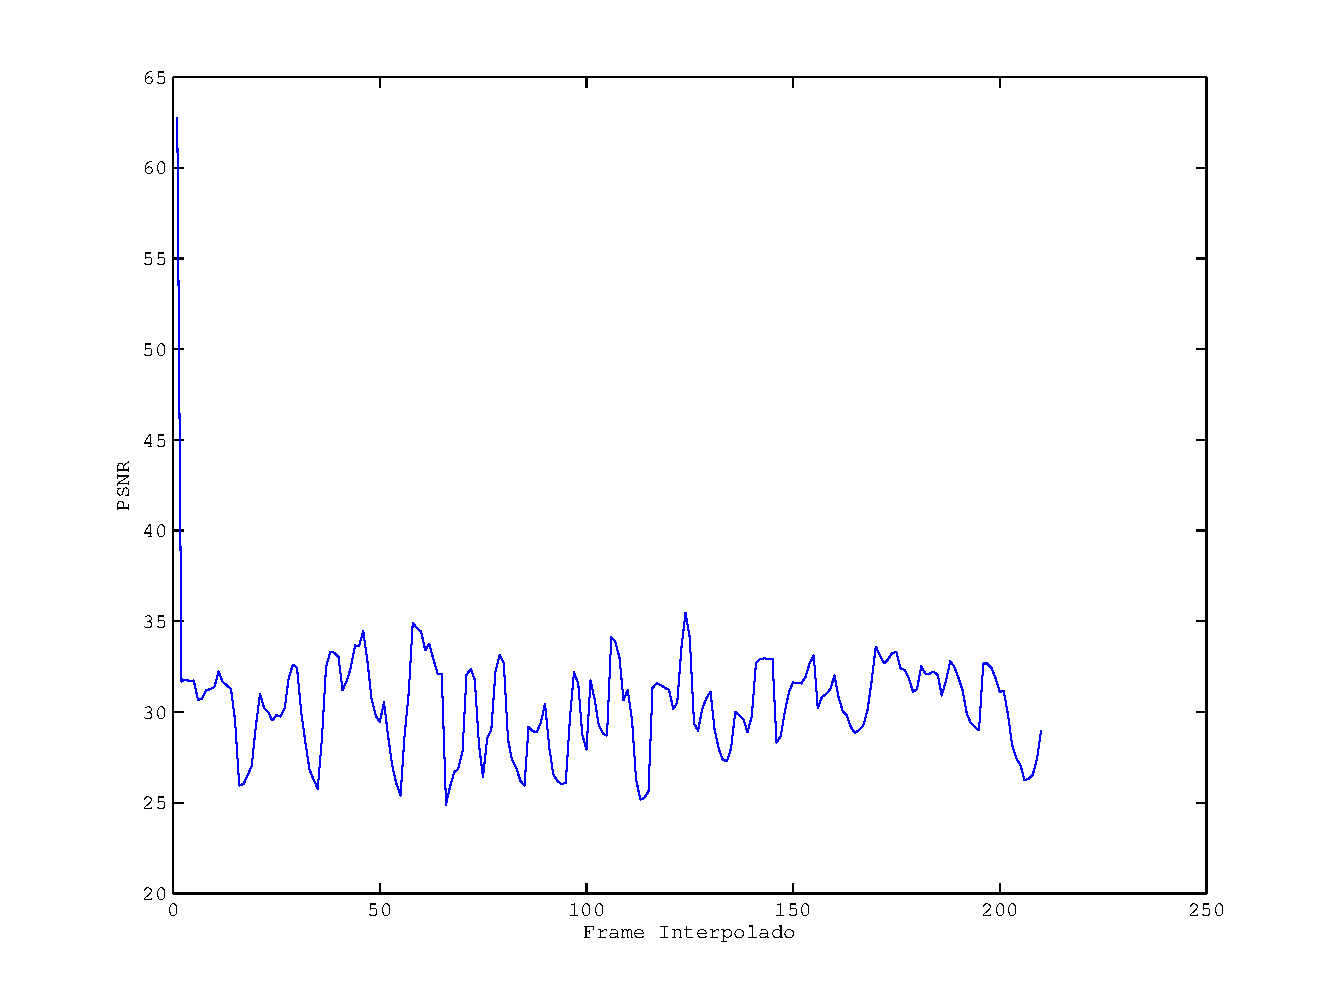
\includegraphics[width=.5\textwidth]{camara_movil-imagen_movil-VECINO-psnr-k10.pdf}
        \label{subfig:movil-movil_vecino-psnr-k10}
    }
    \caption{Comparativa seg\'un cantidad de bloques interpolados}
    \label{fig:movil-movil_vecino-psnr}
\end{figure}

\par Recordando que el PSNR es una m\'etrica inversa del ECM (a mayor PSNR,
menor ECM), observamos que el m\'aximo PSNR para el caso de 10 frames
interpolados (es decir, el m\'inimo ECM) se da en el primer frame. Este PSNR es
claramente un \emph{outlier} respecto de las dem\'as estimaciones, ya que se
puede observar que es claramente mucho mayor a cualquier PSNR de cualquier otro
frame. Y justamente esa estimaci\'on es la que no se observa en el caso de 1
frame interpolado (observar las escalas de los gr\'aficos).

\par Al igual que el caso anterior, esta situaci\'on se di\'o en el primer frame
interpolado. Queda para futuros an\'alisis observar si esto es un patr\'on
consistente y determinar, en tal caso, que es lo que ocurre en los
primeros frames de los videos que generen este comportamiento.

\par Para finalizar el an\'alisis de este m\'etodo, nuevamente se observa el
mismo comportamiento que con spline y la interpolaci\'on lineal respecto de las
regiones que m\'as influyen en el error de la interpolaci\'on (lo cual puede
observarse en el video comparador de \'este
m\'etodo\footnote{\url{https://drive.google.com/open?id=0B0RfkWV-4-XqaEcyVjFDNVpBUFU}})

%---------------------------------------------------------------
\subsubsection{An\'alisis entre M\'etodos}
\par Como en los casos anteriores, a la hora de comparar los distintos
m\'etodos entre s\'i, seleccionamos una \'unica variante del tama\~no de bloque
de splines. Al igual que antes, se decidi\'o tomar la variante que mejores
resultados di\'o en el an\'alisis de dicho m\'etodo, que en el caso de este
tipo de videos es el tama\~no de bloque 8.

\begin{figure}[H]
    \centering
    \subfloat[][PSNR para 2 frames interpolados]{
        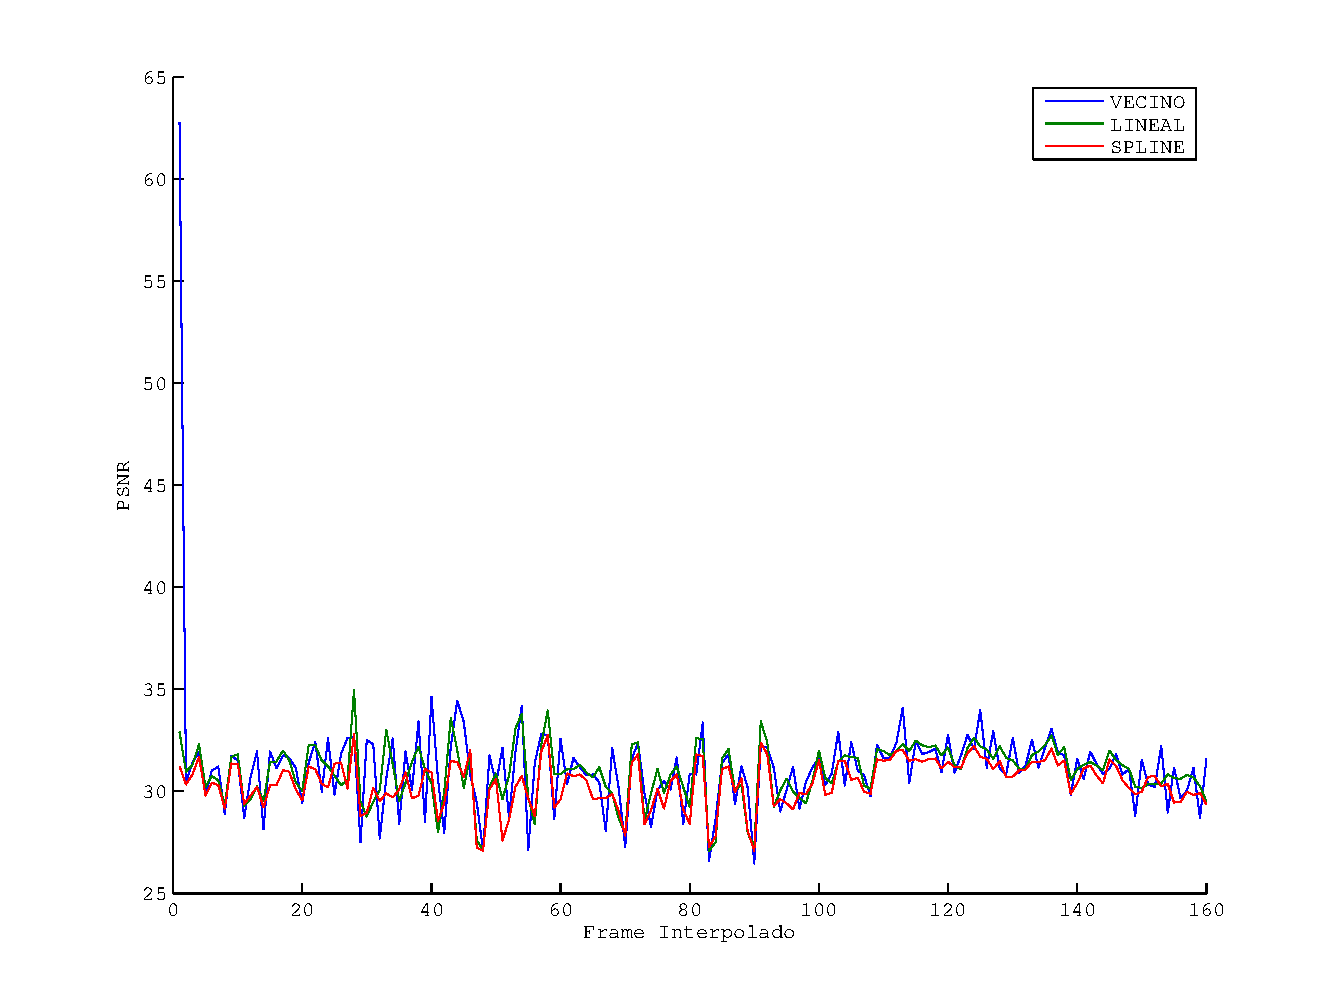
\includegraphics[width=.5\textwidth]{psnr_methods-camara_movil-imagen_movil-k2.pdf}
        \label{subfig:movil-movil_psnr-k2}
    }
    \subfloat[][PSNR para 10 frames interpolados]{
        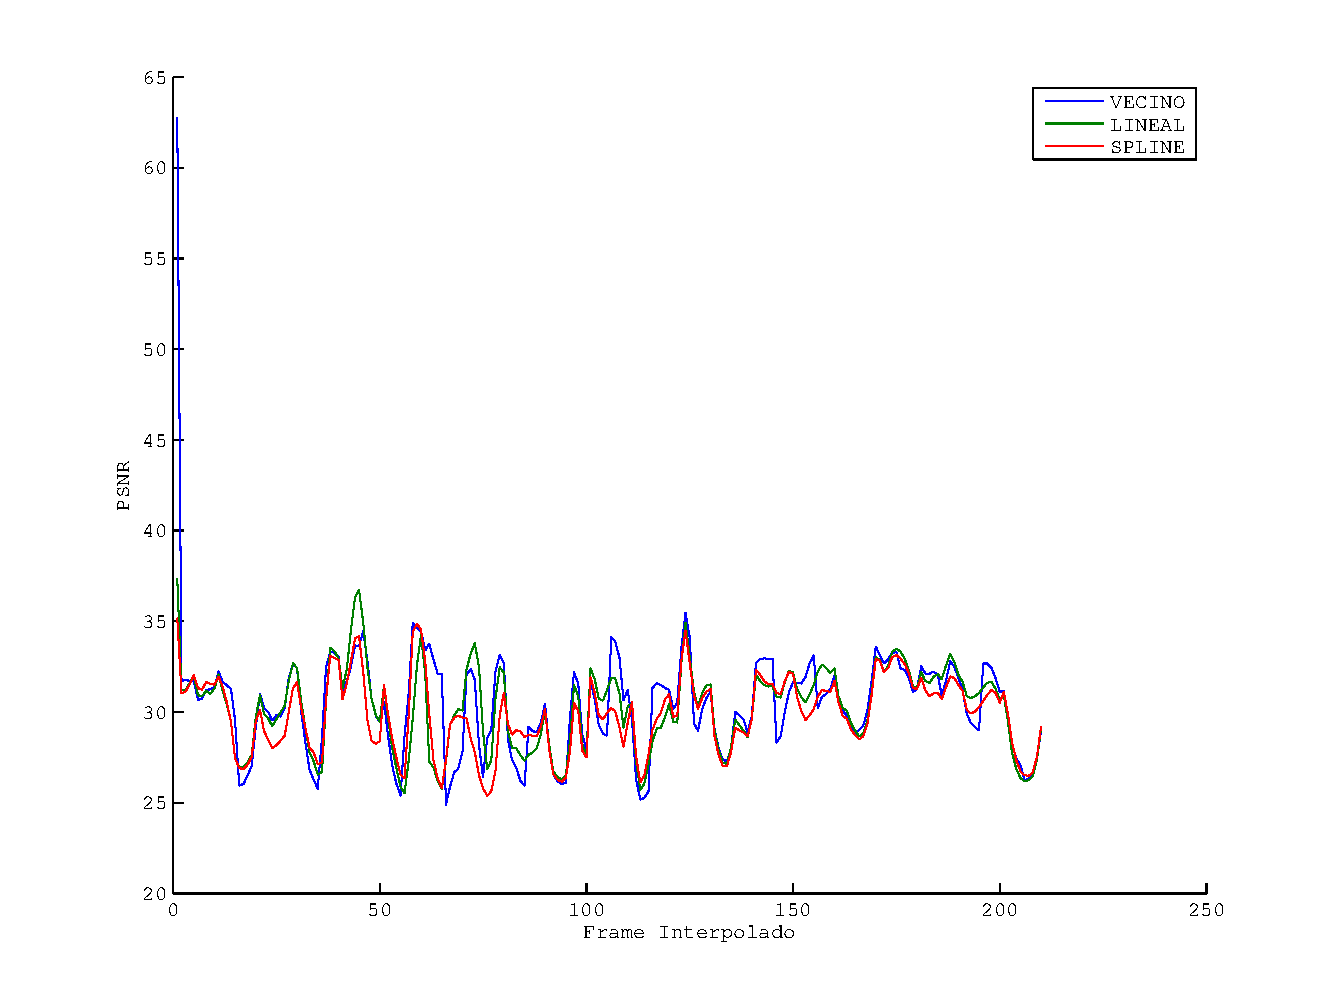
\includegraphics[width=.5\textwidth]{psnr_methods-camara_movil-imagen_movil-k10.pdf}
        \label{subfig:movil-movil_psnr-k10}
    }
    \caption{Comparativa de m\'etodos}
    \label{fig:movil-movil_metodos}
\end{figure}

\par De la comparaci\'on entre m\'etodos del ECM (o PSNR, que de alguna manera
es un poco m\'as claro al normalizar los valores en funci\'on del valor m\'aximo
de un p\'ixel), lo que se observa es que no hay un m\'etodo que sea mejor que
otro de manera m\'as o menos constante. Se observa en la figura
\ref{fig:movil-movil_metodos} que var\'ia constantemente cual es el m\'etodo
con menor y mayor PSNR a medida que avanzan los frames interpolados. Es decir,
\emph{a priori}, ninguno de los m\'etodos tendr\'ia alguna ventaja sobre el
otro.\footnote{No se expusieron los gr\'aficos para las variantes de 1 y 5
frames, ya que las mismas aportan la misma informaci\'on ya expuesta}.

\par Pasamos entonces a analizar los valores estad\'isticos que unifican de alguna
manera las m\'etricas a lo largo de todos los frames.

\par En la figura \ref{fig:movil-movil_methods-mse_estadisticas} podemos observar
el valor medio del ECM. Dicho gr\'afico nos da otra muestra de la paridad de
los m\'etodos para este tipo de videos. Se ve como el ECM medio es similar para
los 3 m\'etodos para todas las variantes de cantidad de frames interpolados.
Existe una ligera ventaja del m\'etodo de interpolaci\'on lineal por sobre los
dem\'as, aunque la misma no es necesariamente significativa.

\par Si nos concentramos ahora en el desv\'io est\'andar, veremos que existe
un patr\'on en el cual el m\'etodo del vecino presenta un mayor desv\'io que
el m\'etodo lineal, y este a su vez mayor que el m\'etodo de spline. Esto, sumado
a lo visto en la figura \ref{fig:movil-movil_metodos}, nos da un patr\'on de
mayor oscilaci\'on del ECM frame a frame para los m\'etodos con mayor desv\'io.
A\'un as\'i, las diferencias entre los desv\'ios para una misma variante de
cantidad de frames interpolados es bastante peque\~na, con lo cual se podr\'ia
decir que los m\'etodos se mantienen similares en este aspecto tambi\'en (con
la excepcci\'on del caso de 1 frame interpolado, donde el vecino m\'as cercano
presenta muchos m\'as picos y oscilaciones que sus contrapartes).

\begin{figure}[H]
    \centering
    \subfloat[][Valor Medio]{
        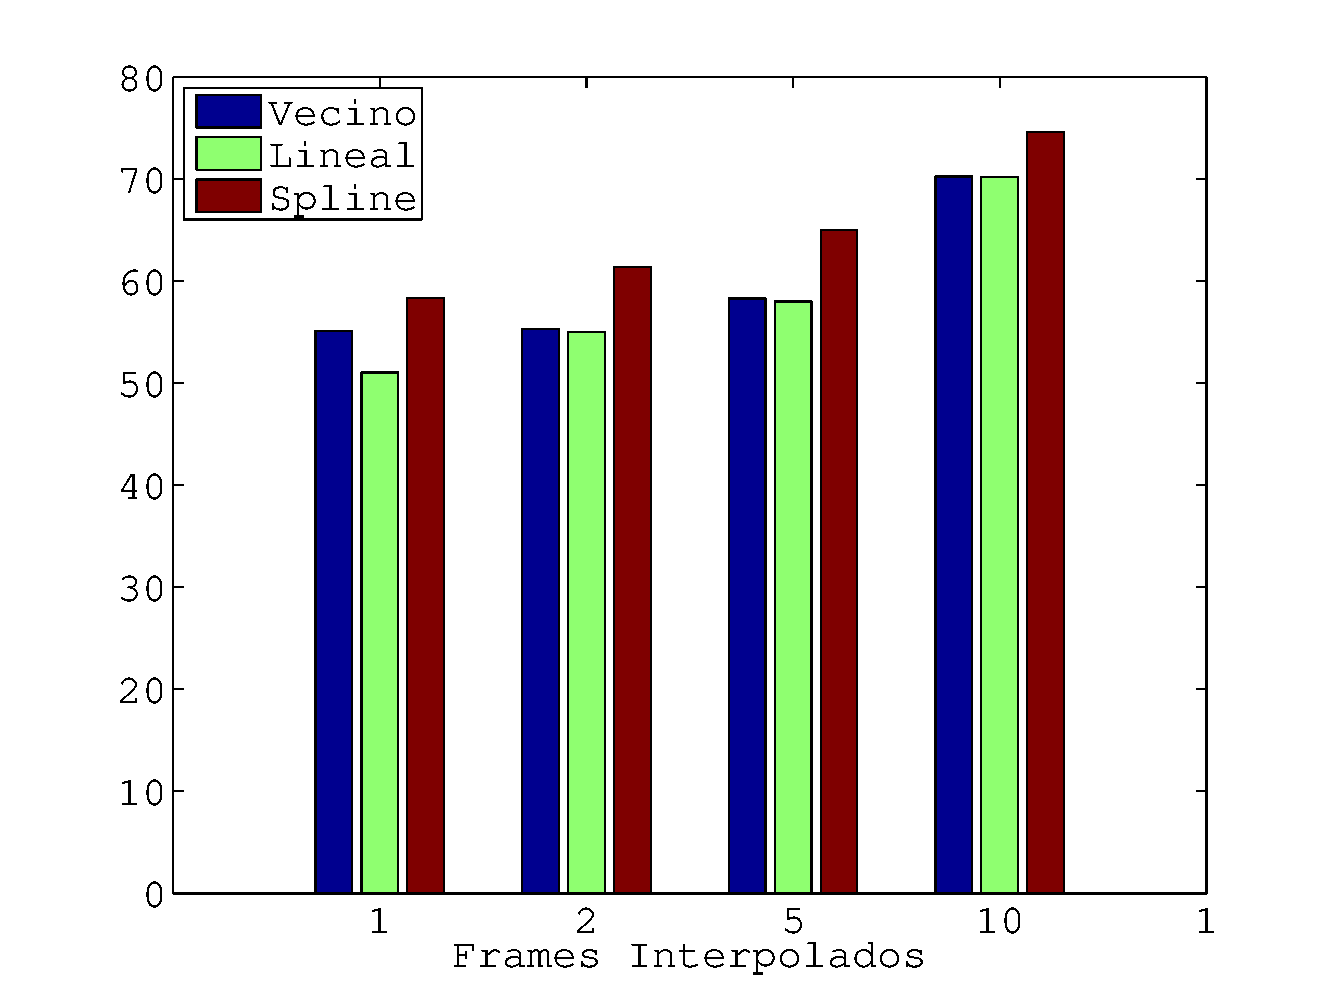
\includegraphics[width=.5\textwidth]{mean_methods-camara_movil-imagen_movil.pdf}
    }
    \subfloat[][Desv\'io Est\'andar]{
        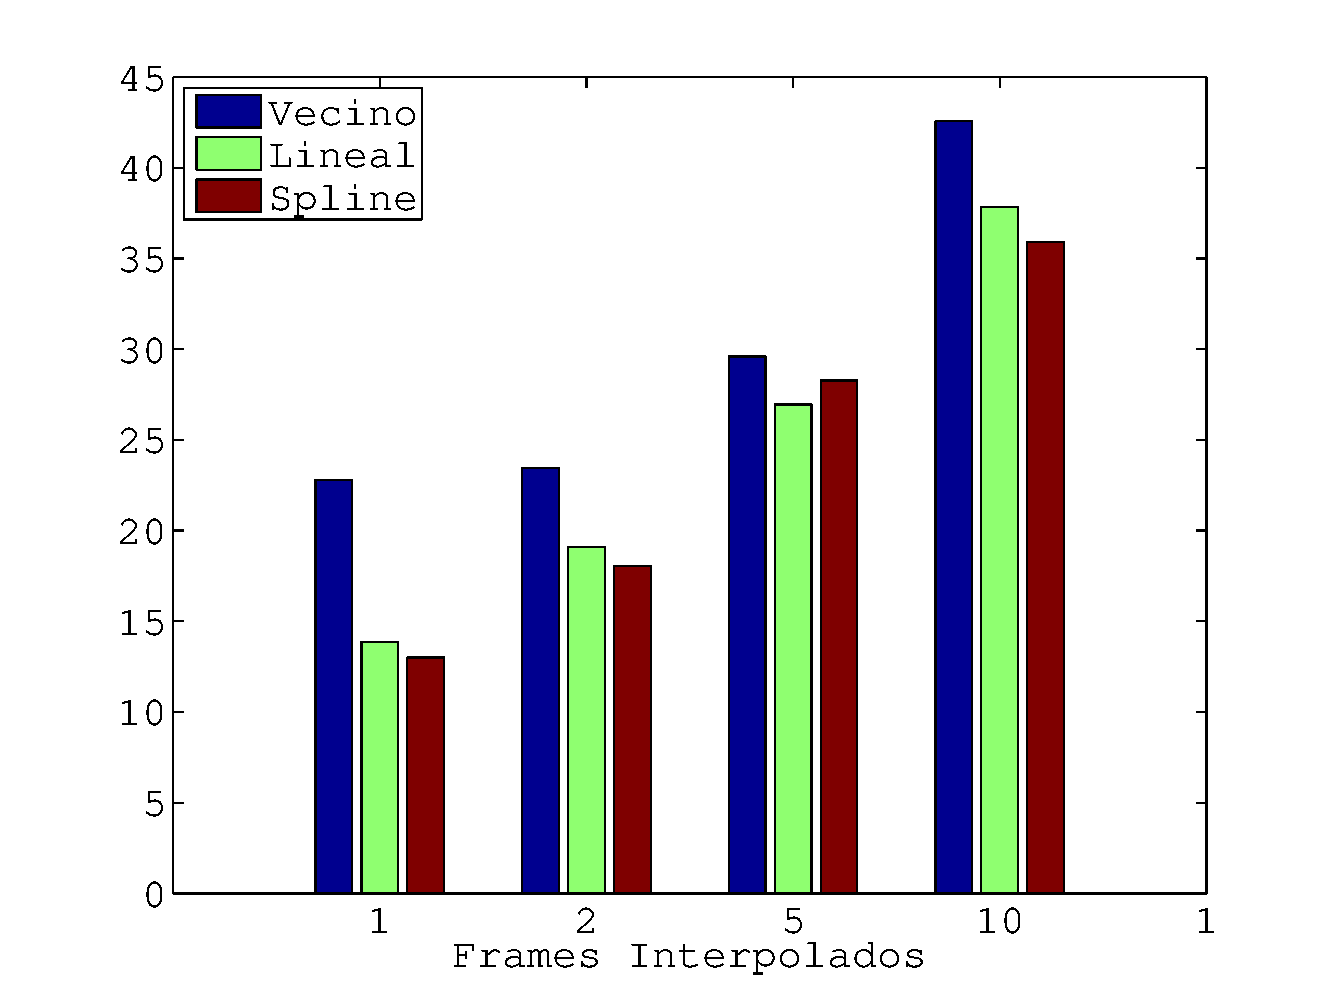
\includegraphics[width=.5\textwidth]{std_methods-camara_movil-imagen_movil.pdf}
    }%\\
    %\subfloat[][M\'aximo]{
    %    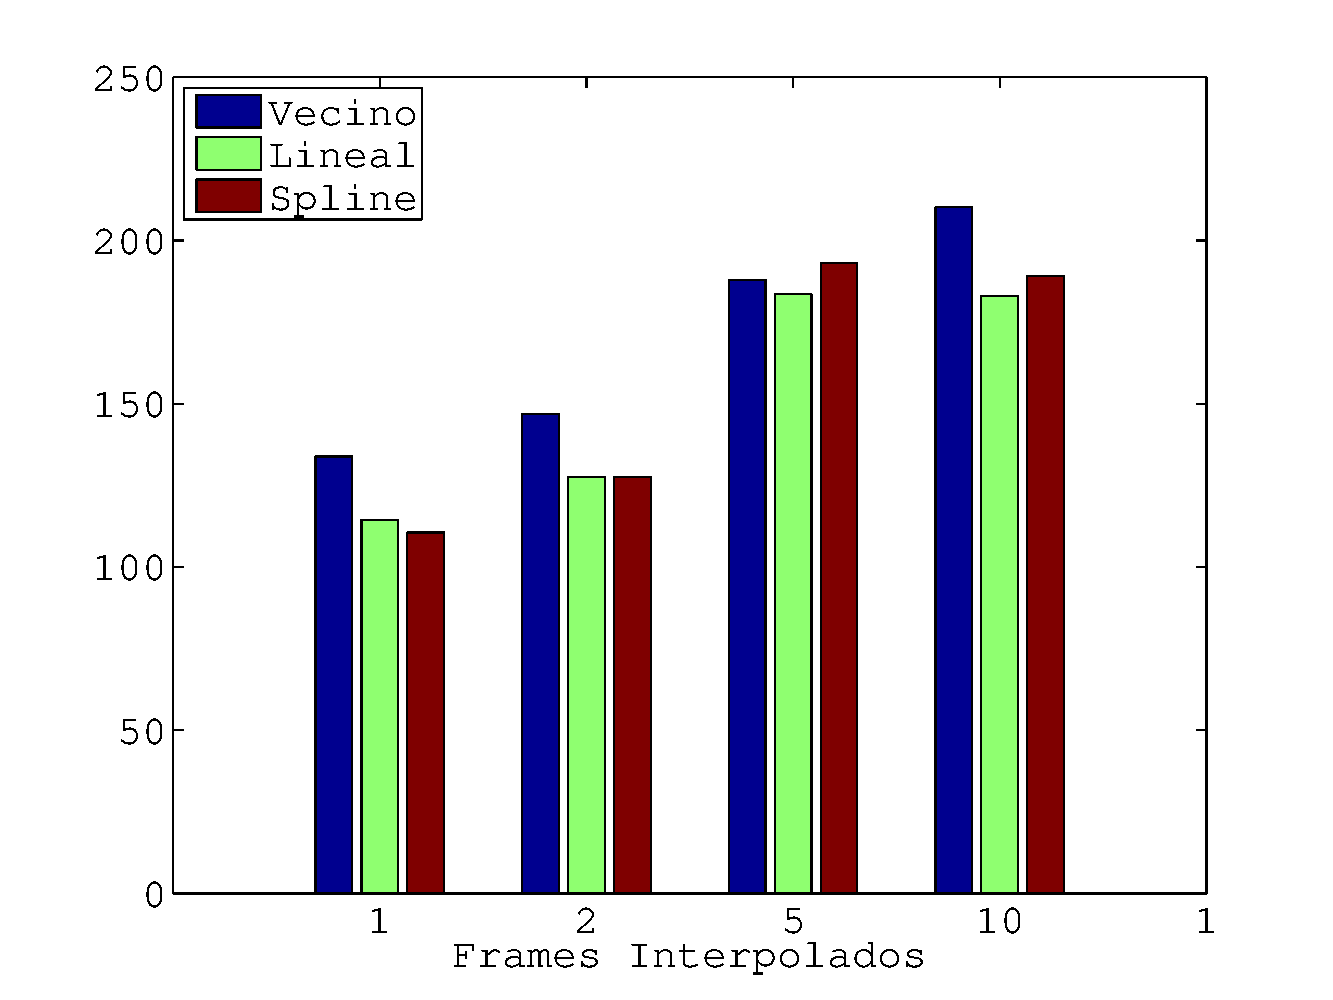
\includegraphics[width=.5\textwidth]{max_methods-camara_movil-imagen_movil.pdf}
    %}
    %\subfloat[][M\'inimo]{
    %    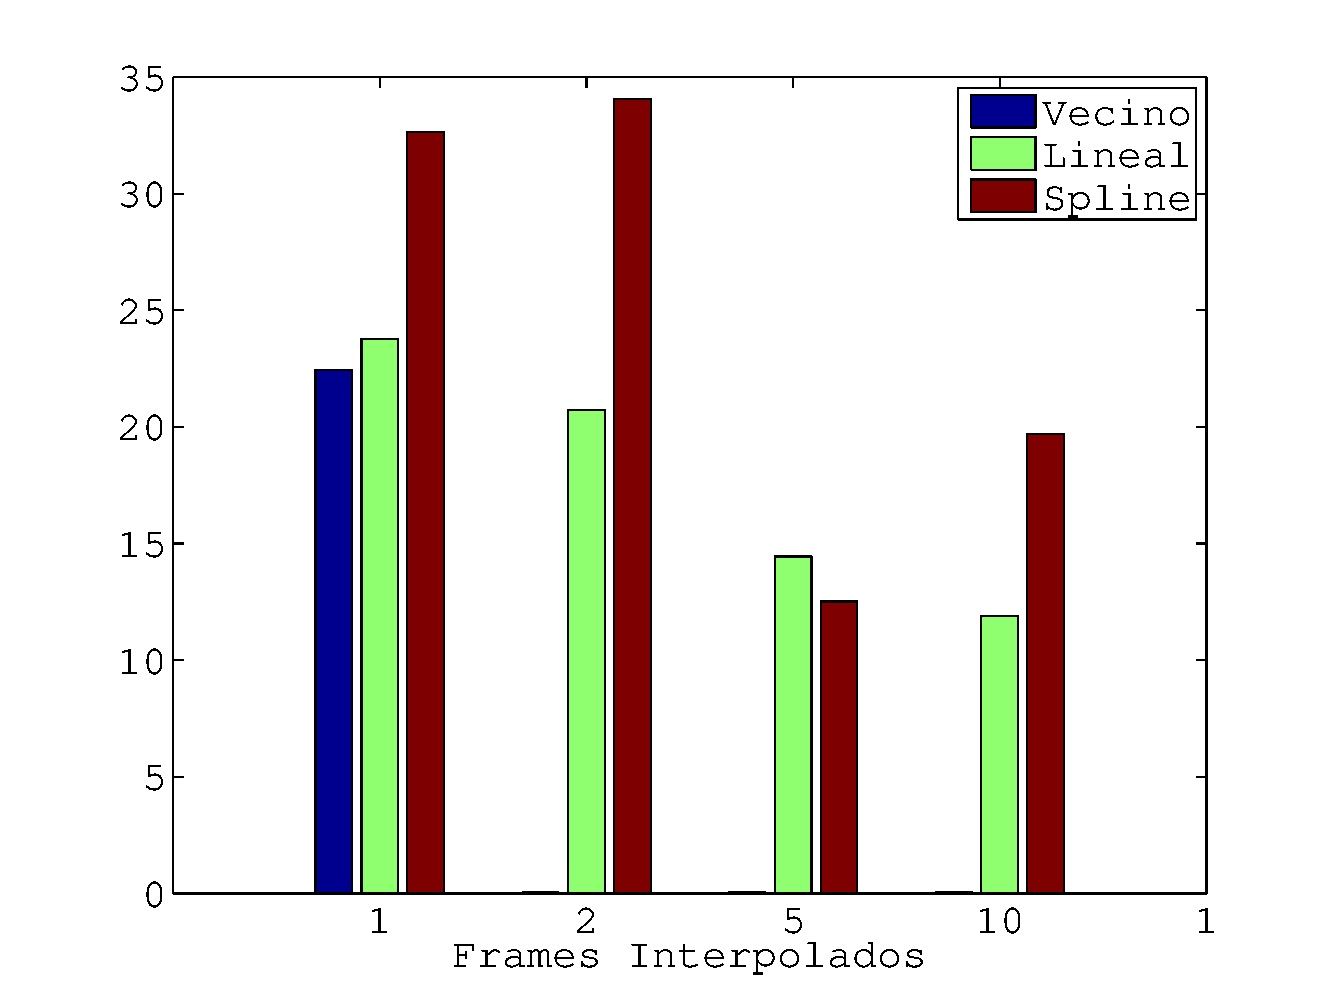
\includegraphics[width=.5\textwidth]{min_methods-camara_movil-imagen_movil.pdf}
    %}
    \caption{Est\'adisticas ECM - Comparativa de M\'etodos}
    \label{fig:movil-movil_methods-mse_estadisticas}
\end{figure}

\par Pasando a observar los videos comparativos de las diferencias entre los
frames interpolados y los originales a los que estiman de los tres m\'etodos,
observamos quelas regiones que m\'as influencia tienen en el error
son las mismas, no cambiando esto de m\'etodo en m\'etodo.

\par En la figura \ref{fig:movil-movil_heatmap} se observan unas capturas de
los videos comparadores de los tres m\'etodos para el mismo frame interpolado.
Si bien el frame en cuesti\'on es interpolado con mayor precisi\'on para el m\'etodo
de spline, seguido por el de interpolaci\'on lineal y por \'ultimo por el vecino
m\'as cercano, el mismo nos sirve para analizar ciertas caracter\'isticas de
la interpolaci\'on de los m\'etodos sobre los frames interpolados.

\par Lo primero que se puede observar es que son mucho m\'as parecidos los frames
interpolados de spline y lineal, donde se observa una superposici\'on con menor
opacidad del frame original siguiente en la reproducci\'on por sobre el frame
original previo. Y en el caso de spline, se ve como un segundo frame superpuesto
a\'un menos opaco (o m\'as transparente). En cambio, en vecino m\'as cercano lo
que se tiene es el siguiente frame original a reproducir, lisa y llanamente.

\par Dado que en la captura utilizada el frame siguiente en la reproducci\'on
esta muy alejado del frame siendo interpolado (estas son capturas para la
variante de 10 frames interpolados), se observa la enorme cantidad de error del
m\'etodo del vecino (debido a que en este experimento, la camara y la im\'agen
siendo capturada tienen mucho movimiento, con lo cual tenemos dos frames
originales usados para realizar la interpolaci\'on extremadamente distintos).
Desde este punto de vista, claramente los m\'etodos de spline e interpolaci\'on
lineal parecer\'ian ser mejores, aunque la simple observaci\'on de los frames
originales e interpolado nos muestra que el resultado no es tan bueno (al menos
para la percepci\'on de los autores). De hecho, el frame interpolado por estos
\'ultimo dos m\'etodos nada tiene que ver con lo que ocurre en el video, y su
efecto en el video es bastante malo de hecho y no necesariamente mejor que el
m\'etodo del vecino m\'as cercano, m\'as allá de que las m\'etricas indiquen lo
contrario (ya de por s\'i los heatmaps de la figura
\ref{fig:movil-movil_heatmap} indican incluso una menor diferencia para lineal
y splines que para el vecino).

\par Nuevamente, en esta captura, observamos que si pensamos que la
representaci\'on del movimiento en un video es el cambio de colores de
p\'ixeles (que pasan a estar en p\'ixeles cercanos), observamos nuevamente en
la figura que el cambio de \'angulo de la c\'amara hace que en un principio se
est\'e enfocando gran parte del cielo (de color claro) para pasar a estar
enfocando gran parte de la cancha de f\'utbol (que es verde oscuro, lo que en
escale de grises se conviernte en un gris muy oscuro comparado contra la
tonalidad del cielo). Y es justamente este cambio el que nos genera m\'as
error, como se puede ver en el gr\'afico de la diferencia entre los frames
original e interpolado. El cielo es la parte que m\'as error aporta en este
frame. As\'i pues, entendemos que lo que m\'as hace fallar a los m\'etodos en
cuesti\'on son los cambios bruscos de un frame a otro de las tonalidades de
cada p\'ixel.

\begin{figure}[H]
    \centering
    \subfloat[][Spline (video entero)]{
        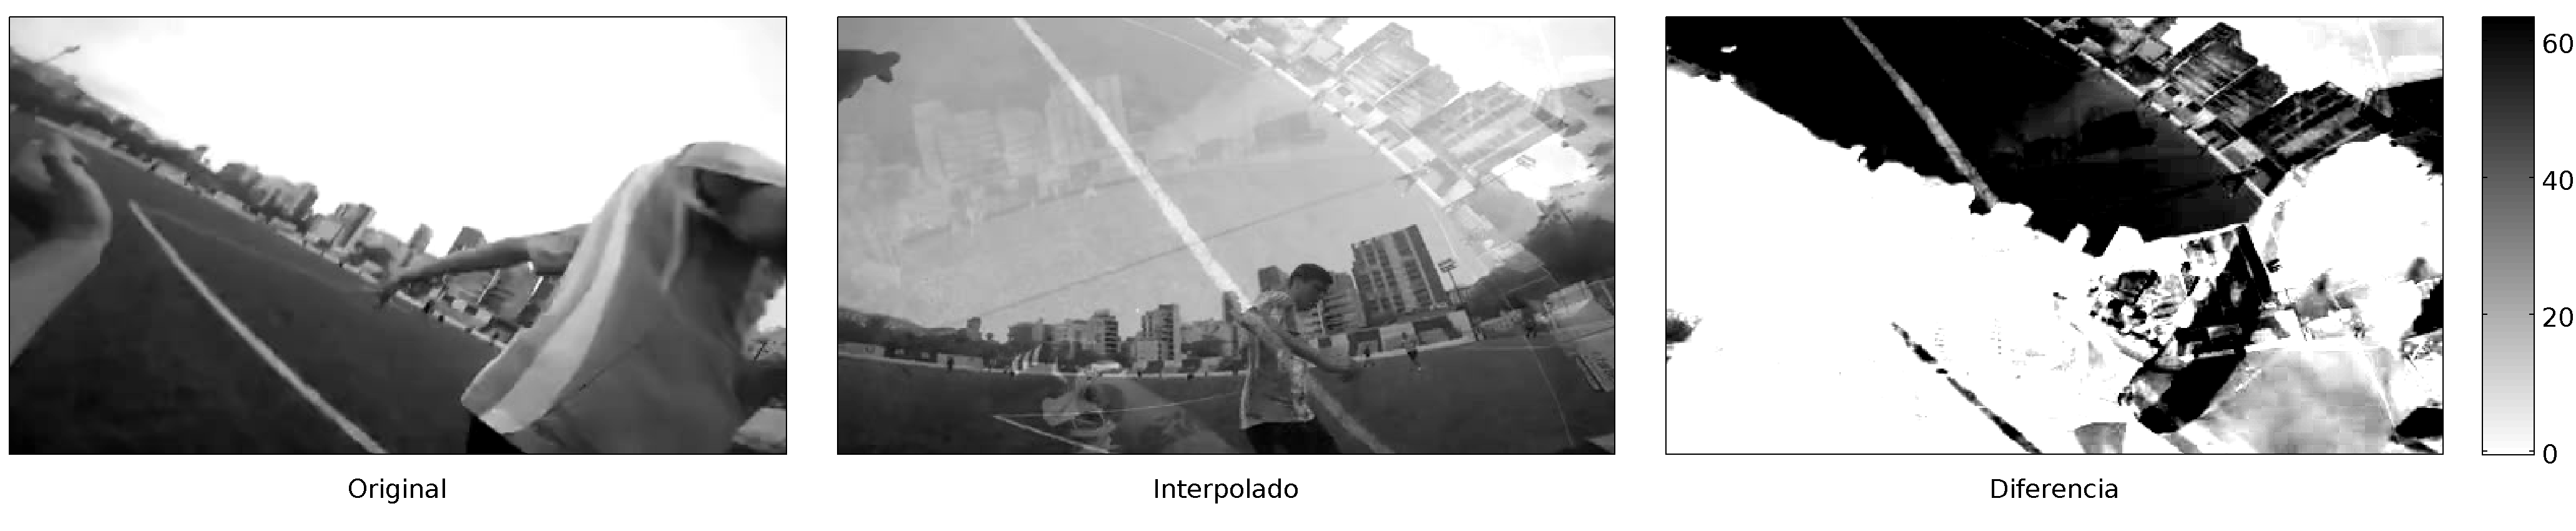
\includegraphics[width=\textwidth]{camara_movil-imagen_movil-spline-k10-blk8.png}
    }\\
    \subfloat[][Interpolaci\'on Lineal]{
        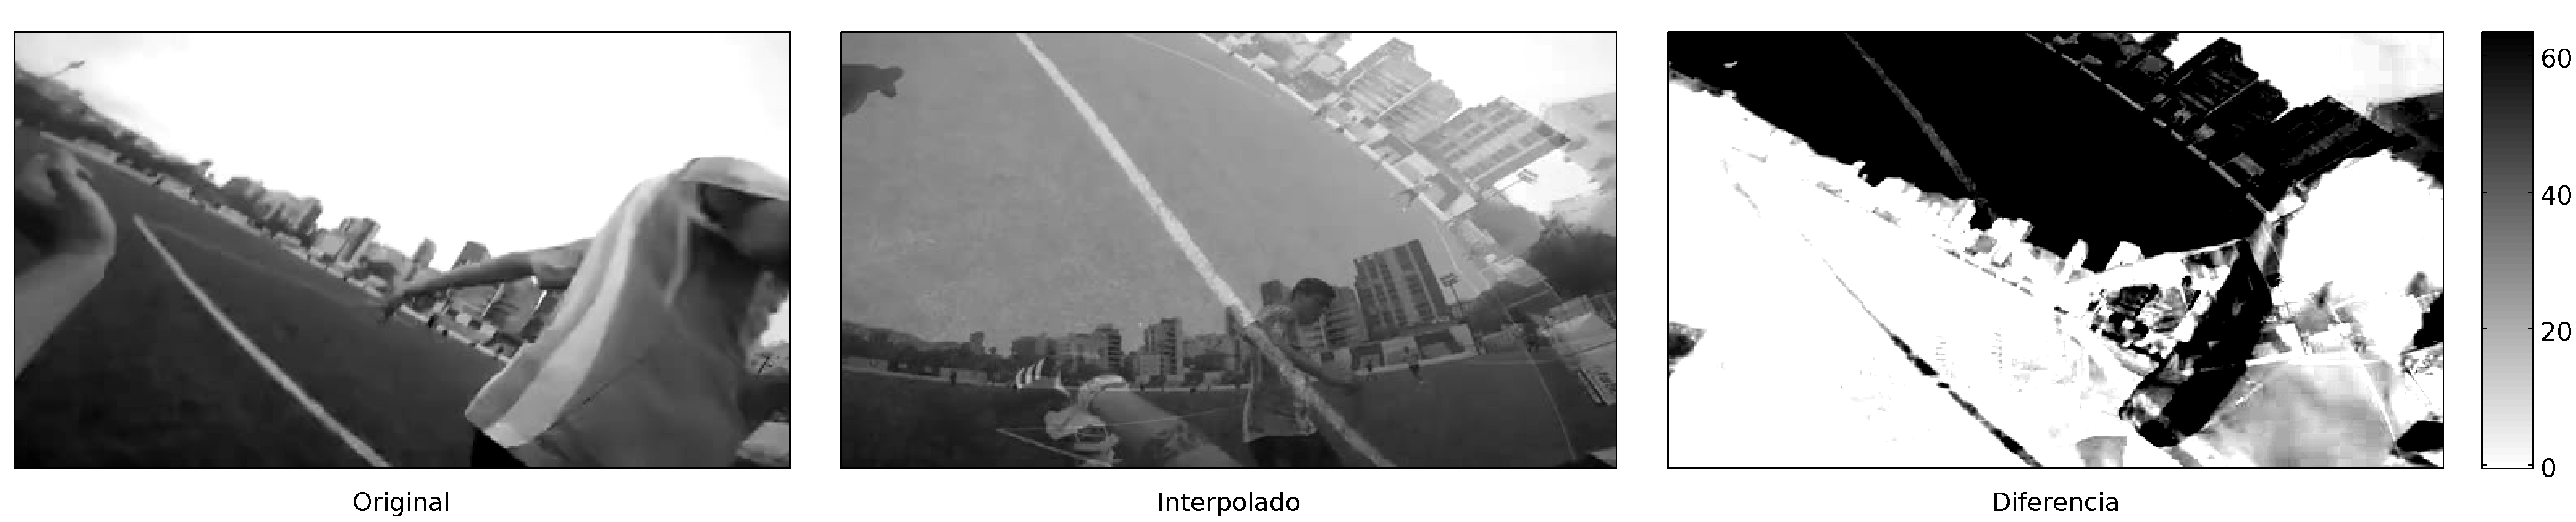
\includegraphics[width=\textwidth]{camara_movil-imagen_movil-lineal-k10.png}
    }\\
    \subfloat[][Vecino m\'as Cercano]{
        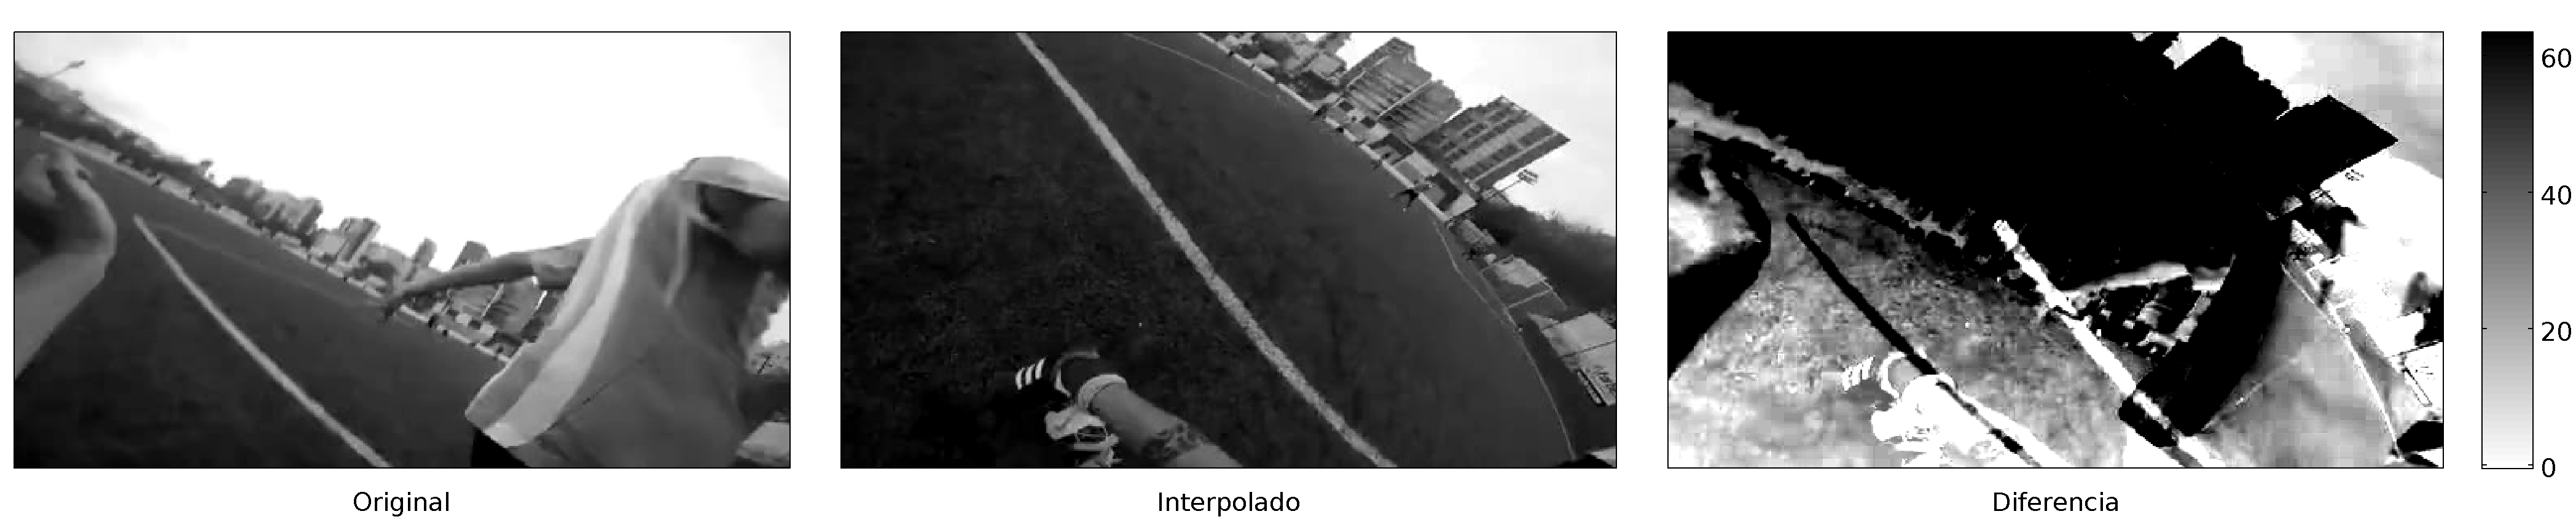
\includegraphics[width=\textwidth]{camara_movil-imagen_movil-vecino-k10.png}
    }
    \caption{Captura del mismo frame de Videos comparativos para interpolaci\'on de 10 frames}
    \label{fig:movil-movil_heatmap}
\end{figure}
%---------------------------------------------------------------
\subsubsection{Conclusiones}
\par A diferencia de otros experimentos, donde de alguna manera se encontraban
aspectos donde los m\'etodos var\'ian de manera significativa, aqu\'i esto
no ocurre (al menos para los aspectos que se decidieron evaluar en este
trabajo).

\par Desprendido de esto, observamos que la diferencia del error cometido por
los m\'etodos para las distintas cantidades de frames interpolados es mucho
menor que para los casos previos. No solo eso, sino que el ECM medio es mayor
que para los casos previos, por m\'etodo y por cantidad de frames interpolados.
B\'asicamente lo que ocurres es que al video presentar tanto movimiento,
tenemos tanto error que ya no importa tanto si interpolamos muchos o pocos
frames, ya que se comete mucho error de cualquier manera (a pesar de que se
cumple la hip\'otesis respecto de que a mayor cantidad de frames se cometer\'a
mayor error).

\par Como resultado principal y global a este tipo de videos, observamos m\'as
que nunca que la gran cantidad de movimientos, y muchos de estos bruscos,
claramente hacen inefectivos a los m\'etodos propuestos para este trabajo. De
hecho, esto se ve reflejado en la opini\'on subjetiva de los autores al
observar los videos interpolados por cualquiera de los m\'etodos. Se dificulta
decidir cual es mejor. En los casos de pocos frames interpolados, cualquiera de
los m\'etodos cumple con las expectativas, pero al aumentar la cantidad de
frames generados artificialmente, todos los m\'etodos se vuelven ineficientes
(quiz\'as en este caso se podr\'ia decir que el efecto logrado por el m\'etodo
del vecino es algo peor\footnote{Subjetividad al mango} que las dos
alternativas evaluadas).

\par Queda para futuros trabajos evaluar estos m\'etodos con videos que se vean
afectados por movimientos de la c\'amara y de las im\'agenes siendo capturadas,
pero donde los movimientos no sean tan bruscos. Quiz\'as en esos casos los
m\'etodos estudiados tengan un comportamiento mejor, ya que demostraron en los
experimentos previos ser m\'as efectivos a la hora de estimar movimientos m\'as
''suaves''\footnote{Por limitantes de tiempo, dichos trabajos no se pudieron
realizar en este trabajo, a pesar de la intenci\'on de los autores.}.

%---------------------------------------------------------------
